%%%%%%%%%%%%%%%%%%%%%%%%%%%%%%%%%%%%%%%%%%%%%%%%%%%
%% Modèle de rapport pédagogique, doublé d'un tutoriel LaTeX
%% Vincent Labatut 2014-20 <vincent.labatut@univ-avignon.fr>
%%%%%%%%%%%%%%%%%%%%%%%%%%%%%%%%%%%%%%%%%%%%%%%%%%%

%\documentclass{ceri/sty/rapport}
\documentclass[full]{ceri/sty/rapport}
%%%%%%%%%%%%%%%%%%%%%%%%%%%%%%%%%%%%%%%%%%%%%%%%%%%
%% Informations générales
%%%%%%%%%%%%%%%%%%%%%%%%%%%%%%%%%%%%%%%%%%%%%%%%%%%

\title{Arkevia Refonte}

\author{Hamza Talaghzi}

%%%%%%%%%%%%%%%%%%%%%%%%%%%%%%%%%%%%%%%%%%%%%%%%%%%
%% Bibliographie
%%%%%%%%%%%%%%%%%%%%%%%%%%%%%%%%%%%%%%%%%%%%%%%%%%%
% Désigne le fichier bibliographique à utiliser
\addbibresource{bibliographie.bib}


%%%%%%%%%%%%%%%%%%%%%%%%%%%%%%%%%%%%%%%%%%%%%%%%%%%
%% Début du document
%%%%%%%%%%%%%%%%%%%%%%%%%%%%%%%%%%%%%%%%%%%%%%%%%%%
\begin{document} 

% Création de la page de titre.
\maketitle

% Justification moins stricte : empêche certains mots de dépasser dans la marge

\sloppy
\phantomsection
\addcontentsline{toc}{section}{Glossaire des acronymes}
\noindent \section*{Glossaire des acronymes}
\markboth{GLOSSAIRE DES ACRONYMES}{}

{
\DefTblrTemplate{head}{default}{}
\begin{longtblr}[label=none,entry=none]{ 
 hlines = {1pt,chambray},
 row{odd} = {bg=azure9},
 row{1} = {bg=azure5, fg=white, rowsep=12pt},
 stretch=1.5,
 colsep=12pt,
 colspec={X[1,l] X[5,l]}
}
\textbf{Acronyme} & \textbf{Désignation} \\
\textbf{API}& \textbf{A}pplication \textbf{P}rogramming \textbf{I}nterface\\
\textbf{B2B} & \textbf{B}usiness \textbf{to} \textbf{B}usiness\\
\textbf{BPO} & \textbf{B}usiness \textbf{P}rocess \textbf{O}utsourcing\\
\textbf{BU} & \textbf{B}usiness \textbf{U}nit\\
 \textbf{CA} & \textbf{C}hiffre d'\textbf{a}ffaires\\
 \textbf{CI/CD} & \textbf{C}ontinuous \textbf{I}ntegration / \textbf{C}ontinuous \textbf{D}elivery\\
 \textbf{CSS} & \textbf{C}ascading \textbf{S}tyle \textbf{S}heets \\
 \textbf{DSI} & \textbf{D}irection des \textbf{S}ystèmes d'\textbf{I}nformation\\
 \textbf{EDI} & \textbf{E}lectronic \textbf{D}ata \textbf{I}nterchange\\
 \textbf{GED} & \textbf{G}estion \textbf{É}lectronique des \textbf{D}ocuments\\
 \textbf{GTA} & \textbf{G}estion des \textbf{T}emps et \textbf{A}ctivités \\
 \textbf{JVM} & \textbf{J}ava \textbf{V}irtual \textbf{M}achine\\
 \textbf{ORM} & \textbf{O}bject-\textbf{R}elational \textbf{M}apping\\
 \textbf{POJO} & \textbf{P}lain \textbf{O}ld \textbf{J}ava \textbf{O}bject\\
 \textbf{QA} & \textbf{Q}uality \textbf{A}ssurance \\
 \textbf{R\&D} &  \textbf{R}esearch and \textbf{D}evelopment \\
 \textbf{RDP} &  \textbf{R}emote \textbf{D}esktop \textbf{P}rotocol  \\
 \textbf{RH} & \textbf{R}essources \textbf{H}umaines\\
 \textbf{SaaS} & \textbf{S}oftware \textbf{a}s \textbf{a} \textbf{S}ervice\\
 \textbf{SASS} & \textbf{S}yntactically  \textbf{A}wesome \textbf{S}tyle \textbf{S}heets\\
 \textbf{SE} & \textbf{S}ystème d'\textbf{e}xploitation\\
 \textbf{SGBDR} & \textbf{S}ystème de \textbf{G}estion de \textbf{B}ases de \textbf{D}onnées \textbf{R}elationnelles\\
 \textbf{SIRH} & \textbf{S}ystème d'\textbf{I}nformation \textbf{R}essources \textbf{H}umaines\\
 \textbf{SRH} & \textbf{S}ervice des \textbf{R}essources \textbf{H}umaines\\
\textbf{UML} & \textbf{U}nified \textbf{M}odeling \textbf{L}anguage 
\end{longtblr}
}
\pageStyleB
%%%%%%%%%%%%%%%%%%%%%%%%%%%%%%%%%%%%%%%%%%%%%%%%%%%
%% Introduction
%%%%%%%%%%%%%%%%%%%%%%%%%%%%%%%%%%%%%%%%%%%%%%%%%%%
\phantomsection
\addcontentsline{toc}{section}{Introduction générale}
\noindent \section*{Introduction générale}
\markboth{INTRODUCTION GÉNÉRALE}{}

\phantomsection
\addcontentsline{toc}{subsection}{Contexte du projet}
\subsection*{Contexte du projet}
Face à la croissance de l'activité de Cegedim SRH, et dans l’optique de garantir un produit de haut qualité, cette dernière a décidé d’adopter une stratégie d’amélioration et d’évolution des systèmes existants.\\

L'un des sujets qualifiés au titre des priorités fut la refonte d'un portail de gestion électronique de documents appelé Arkevia, également connu sous le nom de coffre-fort électronique salarié, un outil de réception et de stockage sécurisé dans lequel le salarié peut stocker ses documents professionnels et personnels : bulletins de paie, ou tout autre document importé au format dématérialisé, pièces d'identités, diplômes, factures, ou autres documents personnel. Ce portail a subi plusieurs changements et évolutions au cours de ces dernières années, rendant l'application volumineuse et difficile à gérer et à comprendre. Malgré les efforts déployés pour maintenir un code modulaire et évolutif, cela n'a pas été suffisant pour réduire la complexité du produit ni à virer les pratiques et méthodes obsolètes ni à corriger les problèmes de performances qui ne cessaient d'augmenter de façon spectaculaire avec le nombre croissant d'utilisateurs.\\

Conscient de ces enjeux, le département R\&D de Cegedim SRH de Rabat a opté pour s'engager dans la refonte de ce portail pour traiter les problèmes et les axes d’amélioration identifiés suite à l’audit architectural réalisé. C'est dans ce contexte que le département R\&D m'a confié ce sujet dont la mission principale est la refonte du portail Arkevia.
\addcontentsline{toc}{subsection}{Objectifs et missions}
\subsection*{Objectifs et missions}
Le stage est axé sur le développement de la refonte de la structure du portail Arkevia afin de répondre aux besoins suivants :
\begin{itemize}
    \item Analyse de l’existant et formalisation du besoin ;
    \item Revue du cœur de l’application et migration vers de nouvelles technologies ;
    \item Restructuration du projet et du mécanisme d'envoi de notifications ;
    \item Réalisation de nouvelles fonctionnalités ;
    \item Adaptation au processus de livraison ;
    \item Réalisation de tests unitaires ;
    \item Rédaction de rapports techniques sur l’avancement du sujet.
\end{itemize}

\subsection*{Contenu du mémoire}
\addcontentsline{toc}{subsection}{Contenu du mémoire}
en cours...
%%%%%%%%%%%%%%%%%%%%%%%%%%%%%%%%%%%%%%%%%%%%%%%%%%%%
%% Présentation de l'organisme d'accueil
%%%%%%%%%%%%%%%%%%%%%%%%%%%%%%%%%%%%%%%%%%%%%%%%%%%
\section{Présentation de l'organisme d'accueil}
\label{sec:presentation}
\addcontentsline{toc}{subsection}{Introduction}
\subsection*{Introduction}
Ce chapitre a pour vocation de présenter l'organisme d'accueil, ses activités et sa structure interne.
\subsection{Groupe Cegedim}
\subsubsection{Présentation}
Fondée en 1969, Cegedim (\textbf{Ce}ntre de \textbf{Ge}stion, de \textbf{D}ocumentation, d’\textbf{I}nformatique et de \textbf{M}arketing) est une entreprise de technologies et de services spécialisée dans la gestion des flux numériques de l’écosystème santé et B2B, ainsi que dans la conception de logiciels métiers destinés aux professionnels de santé et de l’assurance.\\

\begin{figure}[H]
    \centering
    \includegraphics[width=0.25\textwidth]{images/sec1/cegedim-logo.pdf}
    \caption{Logo Cegedim}
\end{figure}

Ses offres s’adressent notamment aux professionnels de santé, industries de santé, laboratoires pharmaceutiques, et compagnies d’assurance. Le Groupe est également présent dans les métiers de la gestion des ressources humaines et de la dématérialisation pour tous types d’industries.
\begin{figure}[H]
    \centering
    \includegraphics[width=0.86\textwidth]{images/sec1/cegedim-ecosystem.pdf}
    \caption{Écosystème Cegedim}
\end{figure}
\subsubsection{Le Groupe Cegedim en quelques chiffres}
Cegedim compte près de 5 300 collaborateurs dans plus de 10 pays (voir figure ~\ref{fig:international_presence}) et a réalisé un chiffre d’affaires de 496.9 millions d’euros en 2020 \cite{cegedim-ca}.
Cegedim SA est cotée en bourse à Paris (EURONEXT : CGM).
\begin{figure}[H]
    \centering
    \begin{subfigure}[t]{0.3\textwidth}
    \centering
        \includegraphics[height=0.28\textwidth]{images/sec1/social-network (1).pdf}
        \caption*{\centering + de \textbf{5 300} collaborateurs}
    \end{subfigure}
   \par\bigskip
    \begin{subfigure}[t]{0.3\textwidth}
    \centering
        \includegraphics[height=0.28\textwidth]{images/sec1/connection.pdf}
        \caption*{Présence dans + de \textbf{10} pays}
    \end{subfigure}
    \hfill
    \begin{subfigure}[t]{0.3\textwidth}
    \centering
        \includegraphics[height=0.28\textwidth]{images/sec1/medal (1).pdf}
        \caption*{\centering \textbf{Top 10} des éditeurs de logiciels français\protect\footnotemark}
    \end{subfigure}
    \hfill
    \begin{subfigure}[t]{0.3\textwidth}
    \centering
        \includegraphics[height=0.26\textwidth]{images/sec1/analytics-market.pdf}
        \caption*{\centering Coté à la \textbf{Bourse} de Paris}
    \end{subfigure}
    \par\bigskip
    \begin{subfigure}[t]{0.3\textwidth}
    \begin{center}
        \includegraphics[height=0.28\textwidth]{images/sec1/ca.pdf}
        \caption*{\centering \textbf{497 M€} de chiffre d’affaires}
    \end{center}
    \end{subfigure}
    \begin{subfigure}[t]{0.3\textwidth}
    \centering
        \includegraphics[height=0.28\textwidth]{images/sec1/data-center.pdf}
        \caption*{\textbf{9} Datacenters}
    \end{subfigure}
    \caption{Groupe Cegedim en chiffres}
    \label{fig:subfigures}
\end{figure}
\footnotetext{Réalisé à partir d’une enquête par questionnaire en ligne. Le Palmarès a été réalisé sur la base des données transmises par chaque entreprise participante, et complétées dans certains cas par des sources extérieures. Certaines données, de nature confidentielle, sont traitées uniquement de façon agrégée. Lire le classement complet sur le site \href{https://www.truffle100.fr/2021.html}{Truffle 100} (publié le 8 juillet 2021).}
\begin{figure}[htb!]
    \centering
    \includegraphics[width=\textwidth]{images/sec1/cegedim-presence-mondiale.pdf}
    \caption{Présence mondiale du groupe cegedim}
    \label{fig:international_presence}
\end{figure}

\subsubsection{Domaines d'activité}
Alliant maîtrise technologique des données, du numérique et des réseaux, les activités du groupe Cegedim se déclinent autour de \textbf{quatre divisions} opérationnelles. Ce découpage vise à améliorer la compréhension des activités en mettant en évidence les différents métiers exercés pour lesquels le lecteur disposera aisément de comparables connus sur le marché.\newline
\fboxsep=10pt\relax\fboxrule=2pt\relax%

\specialbox{white}{actBlue}{40pt}{0.50\textwidth}{
\begin{center}
  \includegraphics[width=0.25\textwidth]{images/sec1/logiciels-et-services.pdf}  
\end{center}
\begin{minipage}{\linewidth}
\footnotesize
regroupe l’ensemble des offres logiciels du Groupe sous toutes leurs formes (licence, SaaS, services internet) ainsi que l’hébergement (agrément HDS) et l‘infogérance. Cegedim cible l’assurance santé et prévoyance (France et Royaume-Uni), les professions paramédicales : kinésithérapeutes, infirmiers, orthophonistes, orthoptistes, podologues, sages-femmes… (France), les directions des ressources humaines (France), les pharmacies indépendantes, groupements ou chaînes de pharmacies (France, Roumanie et Royaume-Uni), les médecins et centres de santé (France, Royaume-Uni, Belgique, Espagne, Italie).
\newline\newline
\end{minipage}
\begin{tblr}
{ 
 rows = {bg=azure9},
 colsep=4pt,
 abovesep=4pt,
 row{2}={abovesep={8pt}},
 colspec={Q[r]Q[l]},
 rowspec={Q[m]Q[m]},
 vline{2} = {2pt,actBlue},
 }
{\Large \textcolor{actBlue}{\textbf{ 277,2 M€}}} &  CA 2020 \\
{\Large \textcolor{actBlue}{\textbf{ 55,8\%}}} &  CA groupe
\end{tblr}
}
\specialbox{white}{actPurple}{40pt}{0.50\textwidth}{
\begin{center}
\includegraphics[width=0.25\textwidth]{images/sec1/data-and-marketing.pdf}
\end{center}
\begin{minipage}{\linewidth}
\footnotesize
regroupe les activités :
\begin{itemize}[leftmargin=*]
    \item Données pour les autorités de santé, les professionnels de santé, les chercheurs, l’industrie de santé et ses partenaires en France, Italie, Allemagne, Espagne, Roumanie et Royaume-Uni ;
    \item Communication en pharmacie et parapharmacie d’enseigne en France sous format papier et numérique ;
    \item Marketing digital auprès des médecins ;
    \item Distribution de produits de santé.\newline\newline
\end{itemize}
\end{minipage}
\begin{tblr}
{ 
 rows = {bg=violet9},
 colsep=4pt,
 abovesep=4pt,
 row{2}={abovesep={8pt}},
 colspec={Q[r]Q[l]},
 rowspec={Q[m]Q[m]},
 vline{2} = {2pt,actPurple},
 }
{\Large \textcolor{actPurple}{\textbf{ 87,8 M€}}} &  CA 2020 \\
{\Large \textcolor{actPurple}{\textbf{ 17,7\%}}} &  CA groupe\\
\end{tblr}
}
\specialbox[t]{white}{actGreen}{40pt}{0.50\textwidth}{
\begin{center}
\includegraphics[width=0.25\textwidth]{images/sec1/flux.pdf}
\end{center}
\begin{minipage}{\linewidth}
\footnotesize
regroupe les activités de gestion du tiers payant (France), de dématérialisation de processus et factures, d’archivage à valeur probante et d’EDI (France, Royaume-Uni, Allemagne). Pour cette activité Cegedim dispose de centres de services en France, Roumanie et Maroc.\newline\newline
\end{minipage}
\begin{tblr}
{ 
 rows = {bg=teal9!50!white},
 colsep=4pt,
 abovesep=4pt,
 row{2}={abovesep={8pt}},
 colspec={Q[r]Q[l]},
 rowspec={Q[m]Q[m]},
 vline{2} = {2pt,actGreen},
 }
{\Large \textcolor{actGreen}{\textbf{ 79,4 M€}}} &  CA 2020 \\
{\Large \textcolor{actGreen}{\textbf{ 16,0\%}}} &  CA groupe
\end{tblr}}
\specialbox{white}{actPink}{40pt}{0.50\textwidth}{
\begin{center}
\includegraphics[width=0.25\textwidth]{images/sec1/BPO.pdf}
\end{center}
\begin{minipage}{\linewidth}
\footnotesize
  regroupe les activités de Business Process Outsourcing en France pour le compte des assureurs complémentaires santé (entre autre gestion des remboursements) et institutions de prévoyance, et départements RH. Pour cette activité Cegedim dispose de centres de services en France et en Roumanie.\\\\
\end{minipage}
  \begin{tblr}
{ 
 rows = {bg=purple9},
 colsep=4pt,
 abovesep=4pt,
 row{2}={abovesep={8pt}},
 colspec={Q[r]Q[l]},
 rowspec={Q[m]Q[m]},
 vline{2} = {2pt,actPink},
 }
{\Large \textcolor{actPink}{\textbf{ 48,9 M€}}} &  CA 2020 \\
{\Large \textcolor{actPink}{\textbf{ 9,8\%}}} &  CA groupe
\end{tblr}
 }
\par\bigskip
\begin{beware}[title=Note : ]
Cette ventilation par division présentée ci-dessus est la typologie privilégiée dans les communiqués de presse et les présentations financières de Cegedim. Il existe encore une cinquième division (non présentée ci-dessus), il s'agit de la division \textbf{Corporate et autres} et regroupe à la fois des activités inhérentes au statut de tête de Groupe coté, et des activités de support aux divisions du Groupe.
Cette division a réalisé en 2020 un chiffre d'affaires de 3,7 millions d'euros
(0,7\% du chiffre d'affaires consolidé du groupe). 

\end{beware}
\subsection{Cegedim SRH}
\subsubsection{Présentation}
Cegedim SRH, filiale du Groupe Cegedim, est l'un des leaders français des solutions et services de gestion de la paie et des ressources humaines. Acteur majeur du Cloud RH et des services externalisés, 
Cegedim SRH dispose d'une expertise de plus de 25 ans dans ce domaine accumulée et reflétée dans sa plateforme \textbf{TEAMS\textsuperscript{RH}} qui offre une large couverture fonctionnelle de solutions dédiées aux Ressources Humaines.\\
\begin{figure}[H]
    \centering
    \includegraphics[width=0.25\textwidth]{images/sec1/cegedim-srh.pdf}
    \caption{Logo Cegedim SRH}
\end{figure}
La société compte parmi ses clients des entreprises nationales et internationales, de tous secteurs d’activité, issues des grands comptes et du mid-market.
\begin{figure}[H]
    \centering
    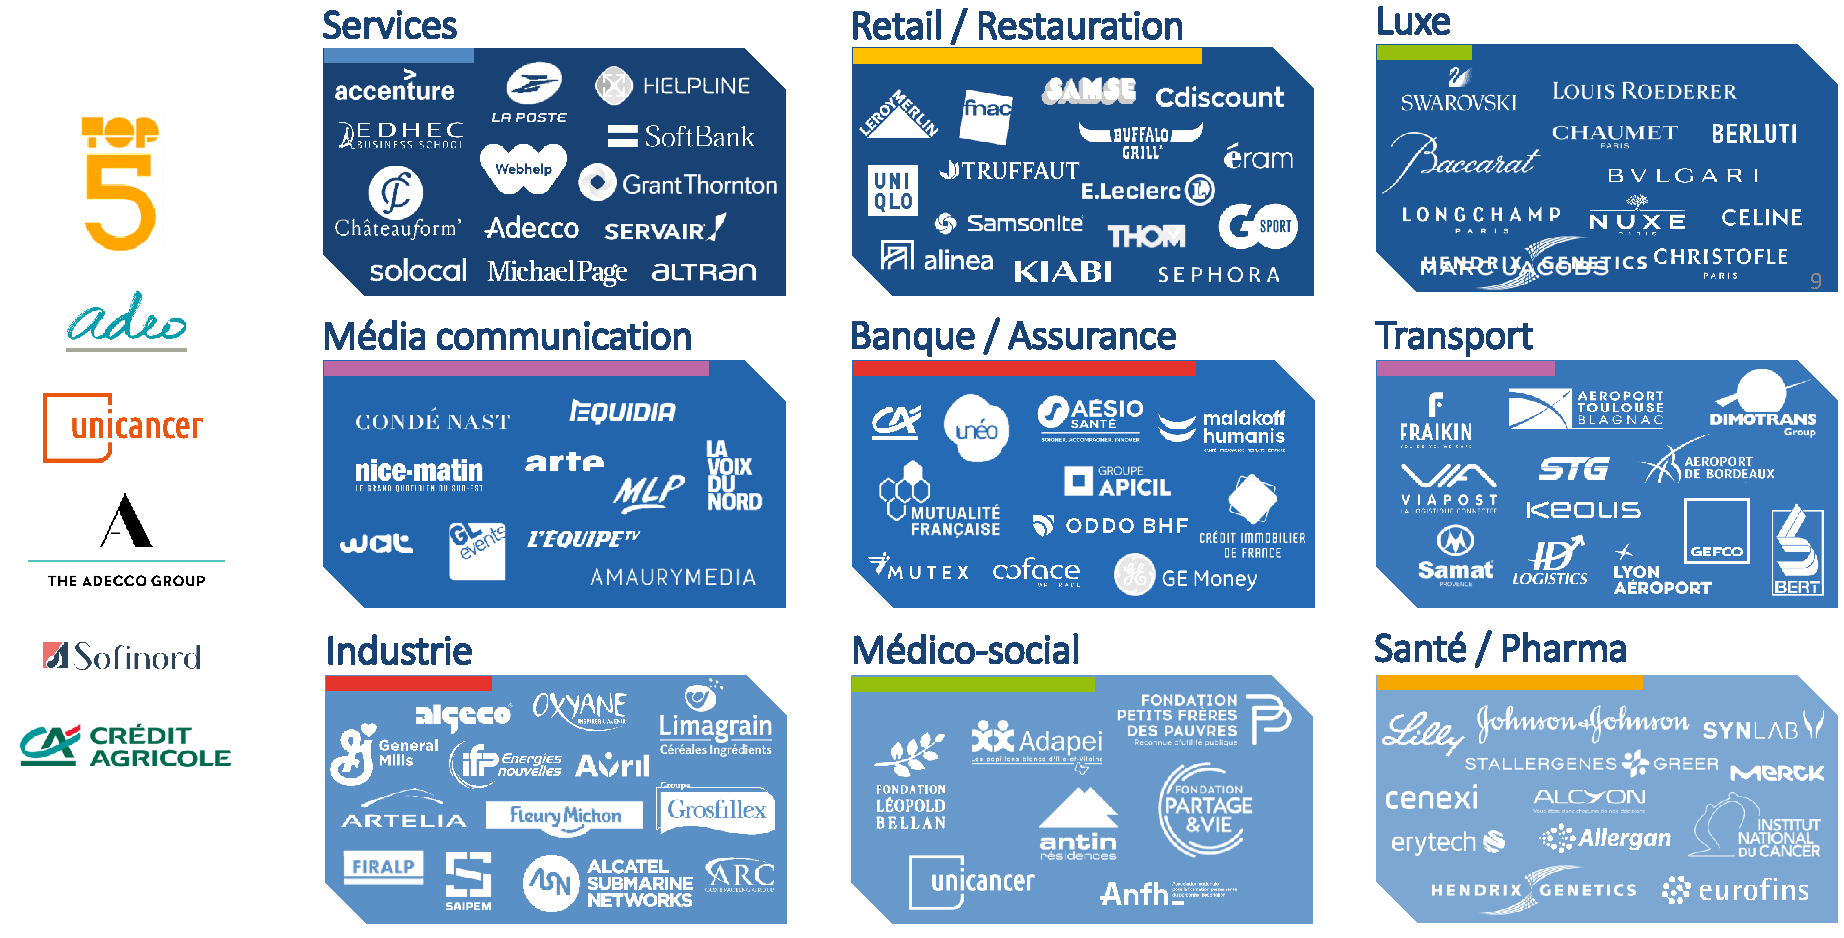
\includegraphics[width=\textwidth]{images/sec1/clients-cegedim-srh.pdf}
    \caption{Clients Cegedim SRH}
\end{figure}
\subsubsection{Domaines fonctionnels}
Capitalisant sur l'apport des nouvelles technologies, Cegedim SRH s'appuie sur un investissement continu et une stratégie de différenciation pour réinventer les outils de gestion RH à travers son offre TEAMS\textsuperscript{RH}, un SIRH complet et modulaire de solutions et services en mode externalisé pour répondre aux besoins d'agilité, de fiabilité et de performance de ses clients.
La plateforme TEAMS\textsuperscript{RH} est constituée d'un ensemble de modules tels que :

\begin{itemize}
    \item paie et gestion administrative,
    \item portail RH collaboratif,
    \item gestion des temps et des activités,
    \item pilotage social,
    \item gestion des RH (Entretiens et Formations),
    \item processus RH dématérialisés intégrés dans la solution (signature électronique et coffres-forts numériques).
\end{itemize}
\newpage
Pour aider ses clients à améliorer la performance de leurs activités, Cegedim SRH propose des services de gestion de la paie et des RH selon quatre niveaux de prestations, en fonction du degré de responsabilité de chaque acteur :\\ 

\vspace*{\fill}
\specialbox{white}{azure5}{40pt}{0.9\textwidth}{
{
\square{azure9}
\color{azure5}
\textbf{SaaS +}\\\\
}
abonnement aux services hébergés de TEAMS\textsuperscript{RH} incluant la maintenance corrective et les mises à jour légales et conventionnelles de l’application.\\}
\par\bigskip
\specialbox{white}{azure5}{40pt}{0.9\textwidth}{
{
\square{azure9} \square{azure8}
\color{azure5}
\textbf{Processing}\\\\
}
externalisation partielle avec pilotage de la relation client, le suivi du traitement de la paie, des opérations d’exploitation, de production et d’éditique.\\}
\par\bigskip
\specialbox{white}{azure5}{40pt}{0.9\textwidth}{
{
\square{azure9} \square{azure8} \square{azure7} 
\color{azure5}
\textbf{BPO on demand}\\\\
}
service d'externalisation de la paie évolutif et sur-mesure.\\}
\par\bigskip
\specialbox[t]{white}{azure5}{40pt}{0.9\textwidth}{
{
\square{azure9} \square{azure8} \square{azure7} \square{azure6}
\color{azure5}
\textbf{BPO}\\\\
}
externalisation complète avec prise en charge de l’ensemble des opérations de traitement de la paie (accréditation ISAE 3402).\\}
\vspace*{\fill}
\clearpage
\subsubsection{Agences et centres de services}
Cegedim SRH dispose de sites de proximité à Paris, Lyon, Lille, Nantes et Toulouse, associés à des centres de développement nearshore à Montargis, Vichy et Genève, et offshore à Bucarest et Rabat (voir figure ~\ref{fig:sites_cegedim}).
\begin{figure}[H]
    \centering
    \includegraphics[width=0.78\textwidth]{images/sec1/cegedim-srh-map2.pdf}
    \caption{Les différents sites SRH}
    \label{fig:sites_cegedim}
\end{figure}
\subsubsection{Organigramme SRH}
Cegedim SRH dispose d’un organigramme qui montre sa structure générale ainsi que l’organisation de ses directions.
\tikzset{
        basic/.style={draw=none, text width=12em, rectangle,font=\bfseries, inner sep=0.25cm, outer sep=0cm,rounded corners=3pt},
        titre/.style={basic, align=center, minimum height=4em, text=azure3, fill=white,draw},
        objectif/.style={basic, align=center, anchor=north, text width=7.5em, minimum height=4.375em, text=azure3, fill=azure9, font=\footnotesize},
        specification/.style={basic, align=left, anchor=center, fill=alice, text width=6.25em, minimum height=3em,text=hoki,font=\footnotesize\bfseries}
    }

\begin{figure}[H]
\centering
 \resizebox{\linewidth}{!}{
   \begin{tikzpicture}[level distance=6em,line width=1pt,gray9,level 1/.style={sibling distance=10em},
    edge from parent path={(\tikzparentnode.south) |- (0em,2em) -| (\tikzchildnode.north)},
    edge from parent/.style={draw},on grid,node distance=2.25cm
    ]% <----- New options on grid and node distance
        \node [titre] {Cegedim SRH}
            child {node [objectif] (o1) {\textbf{Offre et R\&D}}}
            child {node [objectif] (o2) {\textbf{Développement commercial}}}
            child {node [objectif] (o3) {\textbf{Opérations}}}
            child {node [objectif] (o4) {\textbf{Externalisation de services et des TPE/PME}}}
            child {node [objectif] (o5) {\textbf{Satisfaction client et contrôle interne}}}
        ;
        \begin{scope}[every node/.style=specification]
            \node [below=of o1] (o11) {Offre};
            \node [below=of o11] (o12) {Développement technique};
            \node [below=of o12] (o13) {Fonctionnel Paie et\\Juridique};
            \node [below=of o13] (o14) {Fonctionnel RH};
            \node [below=of o14] (o15) {Technique et dev spécifiques};
            \node [below=of o15] (o16) {Qualité \&\\ Documentation};
            \node [below=of o2] (o21) {Marketing\\opérationnel};
            \node [below=of o21] (o22) {Avant-vente};
            \node [below=of o22] (o23) {Chasse};
            \node [below=of o23] (o24) {Parc};
            \node [below=of o3] (o31) {Boulogne};
            \node [below=of o31] (o32) {Lyon};
            \node [below=of o32] (o33) {Nantes};
            \node [below=of o33] (o34) {Lille};
            \node [below=of o34] (o35) {Toulouse};
            \node [below=of o35] (o36) {Centre de \\services};
            \node [below=of o4] (o41) {Rue de la Paye};
            \node [below=of o41] (o42) {BPO Bucarest};
            \node [below=of o42] (o43) {BPO/TPO\\Montargis et Boulogne};
            \node [below=of o43] (o44) {BPO Vichy};
            \node [below=of o44] (o45) {Projets TPO};
            \node [below=of o5] (o51) {Formation};
            \node [below=of o51] (o52) {AMOA et\\Assistance};
            \node [below=of o52] (o53) {RH};
            \node [below=of o53] (o54) {OPEX};
            \node [below=of o54] (o55) {Finances};
            \node [below=of o55] (o56) {Fabex};
        \end{scope}
        \foreach \value in {1,...,6}
            \draw (o1.west) -- ++(-0.5em,0em) |- (o1\value.west);
        \foreach \value in {1,...,4}
            \draw (o2.west) -- ++(-0.5em,0em) |- (o2\value.west);
        \foreach \value in {1,...,6}
            \draw (o3.west) -- ++(-0.5em,0em) |- (o3\value.west);
        \foreach \value in {1,...,5}
            \draw (o4.west) -- ++(-0.5em,0em) |- (o4\value.west);
        \foreach \value in {1,...,6}
            \draw (o5.west) -- ++(-0.5em,0em) |- (o5\value.west);
    \end{tikzpicture}
}
    \caption{Organigramme des Directions Cegedim SRH au 1er janvier 2019}
    \label{fig:organigramme_cegedim_srh}
\end{figure}
\addcontentsline{toc}{subsection}{Conclusion}
\subsection*{Conclusion}
La présentation de l'organisation d'accueil est une étape préliminaire pour introduire l'environnement de notre projet. Dans le chapitre suivant, nous expliquerons en détail l'application sur laquelle portera le travail de refonte.
%%%%%%%%%%%%%%%%%%%%%%%%%%%%%%%%%%%%%%%%%%%%%%%%%%%%
%% Présentation du projet
%%%%%%%%%%%%%%%%%%%%%%%%%%%%%%%%%%%%%%%%%%%%%%%%%%%
%%%%%%%%%%%%%%%%%%
\section{Présentation du projet}
\addcontentsline{toc}{subsection}{Introduction}
\subsection*{Introduction}
Dans ce présent chapitre, nous nous articulerons sur l’étude et l’analyse du projet.
Pour ce faire, nous débuterons par une étude préalable dans laquelle nous exposerons les fonctionnalités de la GED et ses avantages compte tenu de son implication dans le sujet, puis nous entamerons une étude du système existant, pour ensuite identifier les problèmes, les points à améliorer et les solutions envisagées.
\subsection{Étude préliminaire}
Avant d'entamer la discussion sur le sujet du stage, nous allons introduire quelques concepts et terminologie de la GED qui nous aideront à mieux comprendre le sujet par la suite.
\subsubsection{Qu'est-ce que la GED ?}
\begin{beware}[title=Définition : ]
    La GED ou Gestion Électronique de Documents est ensemble de logiciels concourant à réaliser les diverses étapes de la chaîne de traitement d’un document : acquisition, restitution, diffusion \cite{ged}.
    \end{beware}
    La GED est donc un système informatique qui vise à
    gérer et organiser les documents numériques (souvent issus de l'entreprise). En outre, la GED permet la numérisation des documents papier, ainsi que la dématérialisation des processus métier associés.\\La gestion électronique des documents utilise des outils et des fonctionnalités pour gérer toutes les étapes du cycle de vie d'un document numérique :
\begin{itemize}
    \item Création ou acquisition du document (ex : numérisation) ;
    \item Stockage, indexation et organisation du document électronique ;
    \item Gestion de la sécurité des données du document électronique ;
    \item Recherche, consultation du document électronique et échange des informations ;
    \item Archivage électronique du document durant son délai de conservation.
\end{itemize}
\subsubsection{Bénéfices d'une GED}
D’un point de vue stratégique, la mise en place d’une solution de GED rend possible une rationalisation des flux d’informations et donc un gain de temps. Elle permet notamment de :    
\begin{itemize}
    \item Éviter la duplication des processus et ainsi réduire les coûts de traitement.
    \item Éviter la perte de documents.
    \item Trouver facilement et rapidement la bonne version d’un document.
    \item Uniformiser les pratiques documentaires.
    \item Partager des données avec un certain nombre de personnes autorisées.\\
\end{itemize}

D’un point de vue plus opérationnel et technique, la GED garantit : 
\begin{itemize}
    \item La pérennité des documents et de leur support.
    \item L'interopérabilité : les documents peuvent être accessibles sur différentes plates-formes et pour des usages divers.
    \item La sécurité : l’accès aux données est sécurisé, la solution s’adapte aux différents profils utilisateurs.
    \item La traçabilité : retrouver les actions effectuées (dépôts, restitutions, demandes de copies, etc.)
\end{itemize}
\subsection{Étude de l'existant}
\subsubsection{Présentation du projet Arkevia}
\textbf{ARKEVIA} est  un service  innovant  et  pratique de coffre-fort  numérique  développé  par  Cegedim  SRH permettant aux salariés des entreprises adhérentes de recevoir et de conserver dans un espace sécurisé les bulletins de salaire et les communications institutionnelles en version électronique dans des conditions optimales de confidentialité et de sécurité. Arkevia permet également aux salariés de classer et de conserver leurs documents personnels importants tels que les pièces d'identité, les diplômes, les factures, etc.\\

Le coffre-fort Arkevia constitue un espace de stockage sécurisé pour les documents qui y sont déposés (EDI, EDI signé, PDF signé).\\
Il permet de garantir :
\begin{itemize}
    \item \textbf{Intégrité} : L'intégrité des documents, au moyen d’une fonction de signature électronique.
    \item \textbf{Confidentialité} : La confidentialité des documents, au moyen d’une fonction de chiffrement de données.
    \item \textbf{Traçabilité} : La traçabilité des actions effectuées (dépôts, restitutions, demandes de copies, etc.)
    \item \textbf{Vocation probante} : Les solutions de traçabilité constituent de vraies preuves juridiques basées sur leur intégrité, leur exhaustivité et leur opposabilité en cas de litige.\\
\end{itemize}
\newpage
\noindent
\textbf{Bénéfices pour le salarié :}
\begin{itemize}
    \item Accès illimité (24 h/7 j) depuis n’importe quel endroit grâce à une connexion Internet.
    \item Tous les bulletins de salaire déposés dans le coffre-fort ont la même valeur juridique que leur équivalent papier, même en cas de départ de l’entreprise.
    \item Espace personnel sécurisé de 1 Go dédié pour archiver les bulletins de paie et documents RH en version électronique pour une durée de conservation peut aller jusqu'à 50 ans des bulletins de salaire.
    \item Protection des documents importants contre le vol et la perte.
    \item Accès au coffre-fort sécurisé et garanti.\\
\end{itemize}

\noindent
\textbf{Bénéfices pour l’entreprise :}
\begin{itemize}
    \item Optimisation des processus RH d’éditique et de distribution documentaire.
    \item Réduction des coûts de distribution.
    \item Image moderne et innovante de la DRH.
    \item Enrichissement de l’expérience du salarié.
\end{itemize}
\subsubsection{Architecture globale d'Arkevia}
Terminologie nécessaire à la compréhension du sujet :
\begin{beware}[title=Terminologie : ] 
   \begin{itemize}
       \item \textbf{SignArchive} : application de la BU Cegedim e-business, hostée au  datacenter de Boulogne et exploitée par l’équipe interne, ayant pour but le stockage et la signature de documents numériques dans des services à valeur légalement probante.
       \item \textbf{Arkevia} : application Web, décrite dans ce document, présentant une  interface web publique consultable par un navigateur, dont le but est l'exploration et la manipulation de documents dans les coffres SignArchive.
       \item \textbf{Arkevia-SRH} : module d'extension pour Arkevia permettant la mise à disposition dans Arkevia de données (traductions, formulaires d’abonnement, conditions  d'utilisation) issues du système d’information de SRH. Ce module permet la prise en charge des abonnements des utilisateurs d’Arkevia au système de dématérialisation des bulletins de paie émis par SRH.
       \item \textbf{SignArchive-Batcher} : module de traitement générique pour les   applications souhaitant émettre des documents dans SignArchive, à des fins d’exploration par un utilisateur Arkevia.  Le système d’information de SRH utilise SignArchive-Batcher pour placer les bulletins dans les coffres.
   \end{itemize}
\end{beware}
\subsubsubsection{Généralités}
Le développement du produit SignArchive offre à la BU Cegedim e-business, ses clients et partenaires, l’occasion de disposer d’un produit capable à la fois :
\begin{itemize}
    \item de stocker des fichiers (de façon légalement probante si besoin) ;
    \item de les organiser par des métadonnées ;
    \item de fédérer des droits d’accès dynamiques autour de ces fichiers via une API standard (purement HTTP).
\end{itemize}
Au-delà de l’aspect juridique de ce logiciel d’archivage (exploité par les solutions de dématérialisation du groupe), le groupe dispose également d’un moteur de stockage, gestion, recherche et contrôle d'accès qui peut être mis à disposition de toute problématique orientée partage ou publication de document.\\

C’est à une de ces fonctions que s’attache  le projet  Arkevia,  dont  le périmètre fonctionnel est triple :
\begin{enumerate}
    \item Fournir un site web portant une offre de coffre-fort numérique à destination du (grand) public et exposé via le produit SignArchive. Ce site web s’appelle Arkevia.
    \item Offrir à des tiers la capacité de devenir « producteur de documents » pour le portail Arkevia, c’est-à-dire, définir les modalités techniques selon lesquelles un système d’information (interne ou externe) peut s’accrocher au portail Arkevia et à SignArchive,  de façon à ce que les clients d’Arkevia puissent visualiser des documents produits par des tiers.
    \item Implémenter un  tel « tiers producteur » pour les besoins de SRH, permettant la dématérialisation des bulletins de paie émis par l’entreprise.\\
\end{enumerate}

Le deuxième point définit clairement l'objectif d'extensibilité du système, ce qui détermine la plupart des choix de mise en œuvre effectués pour parvenir à la solution globale.

\subsubsubsection{Présentation métier}
La réalisation de la finalité du produit, à   cause de son besoin de généricité, est confiée à trois livrables distincts.
\begin{beware}[title=Note : ]
    La présence de ces trois produits est nécessaire au fonctionnement global de la solution Arkevia+SRH, mais Arkevia peut/aurait pu/pourrait tout à fait exister sans le module SRH, et réciproquement, le module SRH n’a pas besoin d’Arkevia pour pousser les fichiers dans les coffres SignArchive. D’autre part, le module SRH a été développé par Cegedim e-business à la demande de SRH, mais le produit est conçu de sorte qu’Arkevia puisse être implémenté par un producteur qui souhaite prendre en charge lui-même cette implémentation.
\end{beware}
\noindent
Ainsi, les fonctionnalités sont réparties comme suit :\\\\
\textbf{Arkevia}\\
Le site web Arkevia  propose à des navigateurs web en provenance d’internet, la consultation de coffres-forts  SignArchive dans  une interface  de navigation  proche d’un explorateur. Son rôle premier est  donc celui  de « proxy » SignArchive (se connecter pour le compte de l’utilisateur sur SignArchive), et de couche de présentation. D’autre part, Arkevia permet à ses utilisateurs de « s’abonner » à des « producteurs » de documents. La gestion de ces abonnements (présentation  du formulaire d’abonnement spécifique à un producteur, messages de notification du  producteur, ...) nécessite qu’Arkevia puisse communiquer avec le producteur pour échanger images, documents, données, etc. Cette communication doit respecter des principes techniques établis dans le cahier des charges d'implémentation d’Arkevia.\\\\
\textbf{Arkevia-SRH}\\
Ce livrable constitue le module d’abonnement du producteur SRH. Son rôle est :
\begin{enumerate}
    \item De gérer la liste des personnes autorisées à s’abonner au producteur SRH ; et d'en rendre compte à SRH.
    \item De fournir à Arkevia les éléments nécessaires à la  présentation  et la  prise en compte des données d’abonnement (champs de formulaire à  présenter pour s'inscrire, libellés traduits des messages affichés par \textbf{Arkevia} pour le compte de SRH, etc.).
\end{enumerate}

Il est donc constitué à la fois d’une chaîne de traitement chargée de la prise en compte des données d’inscription publiées par SRH, et de web services de publication de données.\\\\
\textbf{SignArchive-Batcher}\\
Ce livrable est une chaîne de traitement publiant, pour le compte de SRH, les bulletins de salaire à dématérialiser dans \textbf{SignArchive}, selon le format admissible pour \textbf{Arkevia}.\\\\
\subsubsubsection{Vue d’ensemble}
Au global, on a une répartition des tâches sous la forme schématique suivante (voir figure  ~\ref{fig:architecture_arkevia}) :
\begin{figure}[H]
    \begin{center}
        \includegraphics[width=\linewidth]{images/sec2/architecture-globale.pdf}
        \caption{Répartition des tâches dans l'écosystème Arkevia}
        \label{fig:architecture_arkevia}
    \end{center}
\end{figure}
\newpage

\begin{enumerate}
    \item  \textbf{Arkevia} se connecte à \textbf{SignArchive} pour en afficher le contenu, indépendamment du fait que SRH publie ou non des documents pour cet utilisateur. Cependant, si l’utilisateur souhaite s’abonner au service de production SRH, alors, Arkevia pousse la demande via un web service au module approprié, \textbf{Arkevia-SRH}.

    \item \textbf{Arkevia-Producteur (Arkevia-SRH)} peut prendre en compte ou non la demande, selon les autorisations qui lui ont été publiées par SRH directement, via le fichier des préinscriptions. Chaque inscription ou résiliation est remontée à SRH via le même canal que le fichier des préinscriptions.

    \item En conséquence de quoi, lors de la fabrication des bulletins de paie, le module de gestion interne à SRH peut constituer une archive des bulletins à archiver conforme aux utilisateurs Arkevia inscrits. Ce fichier est poussé au module \textbf{SignArchive-Batcher} qui pousse les fichiers dans \textbf{SignArchive}.
\end{enumerate}
\subsection{Problèmes et axes d'amélioration}
\subsubsection{Défis technologiques}
Le backend de l'application Arkevia est développé principalement avec la technologie Spring 3.x. Ce framework a été publié pour la première fois en 2004 et a subi de nombreuses révisions depuis lors : 
\begin{itemize}
    \item Spring 2.0 a fourni des espaces de noms XML et le support d'AspectJ ; 
    \item Spring 2.5 a adopté la configuration basée sur les annotations ; 
    \item Spring 3.0 a introduit une solide base Java 5+ à travers le socle du framework et des fonctionnalités telles que le modèle @Configuration basé sur Java.\\
\end{itemize}

Aujourd'hui, le projet Spring et le développement Java ont tous deux évolué de manière significative, incluant à la fois des correctifs de sécurité et de nouvelles fonctionnalités et améliorations, faisant de la migration une tâche assez importante.

À cet égard, il a été convenu de réaliser une étude comparative sur l'impact d'une telle migration du framework Spring ; le résultat de cette étude fera l'objet d'un travail de développement sur la migration du socle technique d'Arkevia.

\subsubsection{Refactorisation et nettoyage du code}
Comme mentionné dans l'introduction, le portail Arkevia a subi plusieurs changements et évolutions au cours des dernières années, rendant le code trop compliqué, redondant et imprégné de mauvaises odeurs (code smells), d'où la nécessité de recourir à un processus de refactoring et d'amélioration du code tout en préservant les fonctionnalités existantes. Le but est de transformer un code inefficace et compliqué en un code plus efficace, de préférence plus simple et plus clair.
\subsubsection{Mécanisme de Notification}
Le mécanisme d'envoi de notifications est responsable de notifier un utilisateur par mail, lorsqu'il y a un nouveau dépôt de document (Bulletin de paie, note de frais, etc.) sur son coffre-fort par la société à laquelle il appartient.\\

Le module de gestion de l'envoi des notifications est intégré à l'application mère Arkevia. Le processus d'envoi est planifié pour être déclenché toutes les deux heures, et à chaque exécution, l'application Arkevia sollicite le service chargé d'interroger l'API SignArchive pour récupérer la liste des documents déposés et celle des utilisateurs associés afin de préluder à l'envoi des notifications.
Le mécanisme actuel n'est pas capable à traiter la volumétrie de documents en production. En effet, ce dernier souffre de plusieurs failles et notamment quand le nombre de documents déposés dans SignArchive est élevé, le système se met à défaillir et à dysfonctionner, ce qui entraîne que certains utilisateurs ne reçoivent plus les notifications sur la présence des documents déposés dans leur coffre-fort ou les reçoivent plusieurs fois pour un même document, etc. 

\subsection{Objectif de la refonte}
Après avoir introduit l'application existante et repéré les différents points d'amélioration et les problèmes engendrés au sein de cette dernière, nous procéderons à une refonte globale de l'application dont l'objectif sera de revoir, corriger et améliorer ces aspects recensés afin notamment de rendre l'application plus performante, facile à maintenir et à faire évoluer.


\addcontentsline{toc}{subsection}{Conclusion}
\subsection*{Conclusion}
Dans ce chapitre, nous avons décrit de manière didactique l'application qui fera l'objet de la refonte, et ce, afin d'exposer le contexte global de notre projet en dégageant les problématiques et les différents axes d'amélioration. Enfin, nous avons clôturé ce chapitre en exprimant l'objectif de la refonte auquel s'articule le sujet de l'étude.

%%%%%%%%%%%%%%%%%%%%%%%%%%%%%%%%%%%%%%%%%%%%%%%%%%%%
%% Éléments flottants
%%%%%%%%%%%%%%%%%%%%%%%%%%%%%%%%%%%%%%%%%%%%%%%%%%%
%%%%%%%%%%%%%%%%%%
\section{Méthodologie de gestion du projet}
\subsection{Introduction}
\subsection{étude préliminaire}
\subsubsection{Cycle de vie de logiciel}
\subsubsection{Comparaison des différents méthodes de développement}
\subsection{Conduite de projet}
\subsubsection{Processus de livraison adopté par Cegedim SRH}
\subsubsection{Déroulement du projet}
scrum
\subsubsection{Processus de développment}
\subsubsection{Gestion du flux git avec Git-flow}
\subsection{Planification et suivi du projet}
\subsubsection{Diagramme de Gantt}
Le diagramme de gantt:\\
\begin{figure}[H]
    \begin{center}
        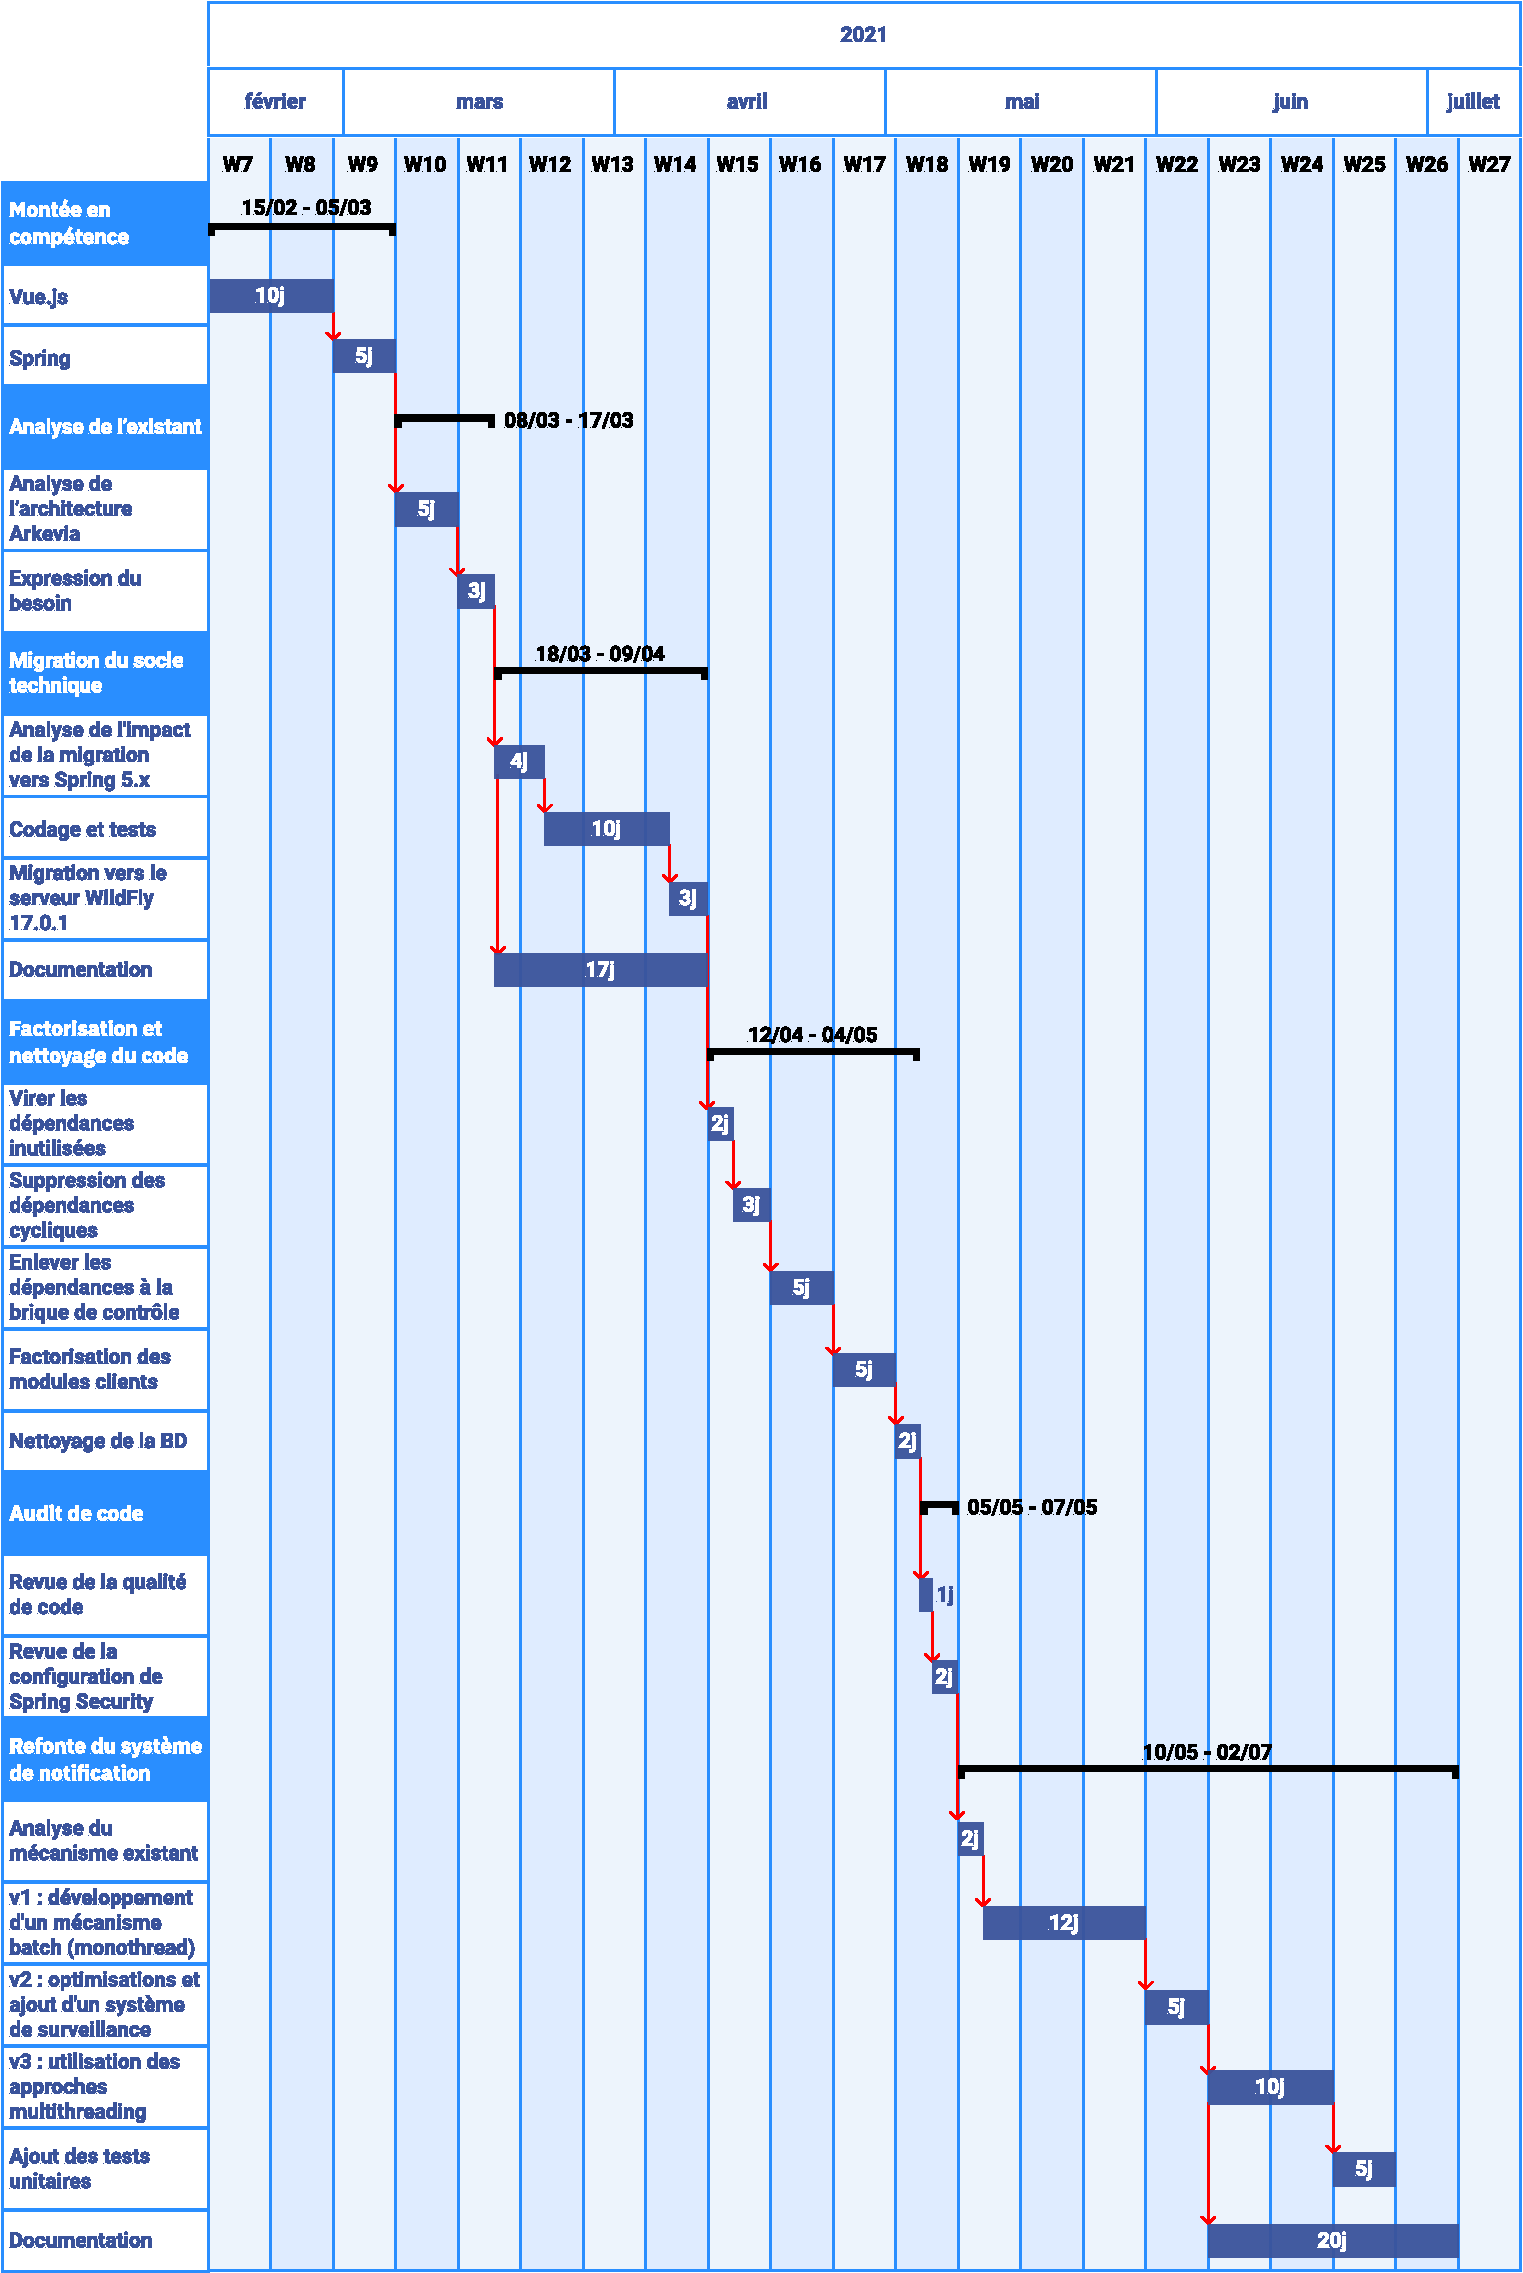
\includegraphics[width=\linewidth]{images/sec3/gantt.pdf}
        \caption{Diagramme de Gantt}
    \end{center}
\end{figure}
\subsection{Conclusion}
%%%%%%%%%%%%%%%%%%

%%%%%%%%%%%%%%%%%%%%%%%%%%%%%%%%%%%%%%%%%%%%%%%%%%%%
%% Conceptions et spécification des besoins
%%%%%%%%%%%%%%%%%%%%%%%%%%%%%%%%%%%%%%%%%%%%%%%%%%%
\section{Conceptions et spécification des besoins}
\addcontentsline{toc}{subsection}{Introduction}
\subsection*{Introduction}
\subsection{Étude conceptuelle du système}
Cette section a pour objectif de présenter une conception détaillée du portail arkevia (l'existant), afin de bien comprendre son fonctionnement et de se familiariser avec le sujet.
\subsubsection{Méthodologie de conception}
Afin de modéliser et décrire les différents aspects de notre système, nous utiliserons le langage
graphique de modélisation unifié UML 2.0.\\
UML est un langage formel et normalisé en termes de modélisation objet. Son indépendance par rapport aux langages de programmation, aux domaines d’application et son caractère polyvalent ont fait de lui un langage universel. Il fournit un moyen astucieux permettant de représenter diverses projections, grâce aux diagrammes.\\\\
Les diagrammes sont représentés sous deux types de vue :
\begin{itemize}
    \item D’un point de vue \textbf{statique} ou \textbf{structurelle} du domaine avec les diagrammes de structure (Structure Diagrams).
    \item D’un point de vue \textbf{dynamique} avec les diagrammes de comportement (Behavior Diagrams) et les diagrammes d’interactions (Interaction Diagrams).\\
\end{itemize}

L’utilisation itérative des outils UML dans l’analyse et la conception, permet d’obtenir une meilleure compréhension de la configuration système requise et les processus à exécuter dans le système pour répondre à ces exigences.\\
La première itération d’analyse devrait se situer à un niveau très élevé afin d’identifier
les objectifs généraux du système et de valider les exigences au moyen d’une analyse du
cas d’utilisation. L’identification des acteurs et la définition du modèle de cas d’utilisation
initial font partie de cette première itération. Les itérations d’analyse ultérieures affinent
davantage la configuration système requise en développant des scénarios de cas d’utilisation, des diagrammes de classes, des diagrammes de séquence, des diagrammes d’états, etc. Chaque itération prend successivement plus en détail la conception du système jusqu’à ce que les objets et les relations dans le système soient clairement et précisément définis dans les diagrammes UML.\\

Une fois l’analyse et la conception terminées, nous disposerons d’une vue globale,
détaillée, et précise sur l’ensemble des spécifications pour les classes, les scénarios, les
activités et le séquencement dans le système. En général, un lien peut être établi entre
la rigueur de l’analyse et de la conception d’un système, le temps nécessaire pour le
développer, et la qualité du produit livré en conséquence.\\
\begin{beware}[title=Conclusion : ]
L’UML propose des diagrammes pour décrire les différents aspects d’application mais
ne précise pas la séquence d’étape à suivre ou la démarche à suivre pour la réalisation de
ces diagrammes. Un processus de livraison est alors nécessaire (voir section ).
\end{beware}

\subsubsection{Identification des acteurs}
Un acteur représente un rôle c’est à dire une personne, un matériel ou un logiciel qui
interagit directement avec le système. Les acteurs pouvant interagir avec l’application
sont :
\begin{itemize}
    \item \textbf{Employeur} : Personne morale adressant aux utilisateurs des documents.
    \item \textbf{Titulaire} : Salarié, actuel ou passé, de l’Employeur ayant ouvert et utilisant le coffre-fort électronique.
    \item \textbf{Utilisateur} : Titulaire ou, le cas échéant, les personnes physiques spécifiquement habilitées par le Titulaire.
    \item \textbf{Opérateur} : Personne morale qui met en œuvre un service de coffre-fort électronique et règle le fonctionnement opérationnel du système et des mesures de sécurité afférentes, en l’espèce CEGEDIM SRH. 
\end{itemize}

\subsubsection{Diagramme de cas d'utilisation général}
Le diagramme de cas d'utilisation représente la structure des grandes fonctionnalités nécessaires aux utilisateurs du système. C'est le premier diagramme du modèle UML,
celui où s'assure la relation entre l'utilisateur et les objets que le système met en oeuvre.\\
Un cas d'utilisation est une description de l'application qui privilégie le point de vue de l'utilisateur. Il décrit de façon graphique et/ou éventuellement textuelle comment un acteur va utiliser l'application pour atteindre un objectif.
\begin{figure}[H]
    \includegraphics[width=1.1\linewidth]{images/sec3/usecase.pdf}
    \caption{Diagramme de cas d'utilisation général}
\end{figure}
\footnotetext[1]{représente le cas d'un acteur (non propriétaire) autorisé à utiliser le compte.}
\newpage
\subsubsection{Raffinement des cas d'utilisation prioritaires}
\definecolor{arkevia-btn-border}{HTML}{a3d7de}
\definecolor{arkevia-btn-bg}{HTML}{1aa1b4}
\definecolor{arkevia-btn-bg2}{HTML}{453659}
\setlength{\fboxrule}{1pt}
\setlength{\fboxsep}{6pt}

\begin{longtblr}[caption={Description textuelle du cas d’utilisation « S'inscrire »},
    note{1} = {Le mot de passe doit comporter un minimum de 8 caractères et un maximum de 20 caractères, au moins une lettre, au moins un chiffre, au moins un caractère spécial parmi @\#\$\%\^\&+=?\_|!,;.:\/ et ne doit pas contenir d'espaces.}]{
    hlines = {0.5pt,chambray},
    vlines = {0.5pt,chambray},
    row{odd} = {bg=azure9},
    colsep=4pt,
    rowsep=4pt,
    colspec={Q[l]X[l]},
    rowspec={Q[m] Q[m] Q[m] Q[m] Q[m] Q[m]},
}
\textbf{Acteur} & Salarié (Titulaire) \\
\textbf{Objectif}& 
L'inscription permet aux salariés d'activer la mise à disposition de leurs bulletins de paie électroniques dans leurs coffres-forts.\\
\textbf{Pré-condition} & 
Disposer d'une connexion Internet et d'un navigateur.\\
\textbf{Scénario} & 
\begin{minipage}{\linewidth}
\raggedright
\begin{enumerate}[leftmargin=*]
    \item Le salarié se rend sur \url{www.myarkevia.com} à l'aide d'un navigateur.
    \item Le salarié clique sur \fcolorbox{arkevia-btn-border}{arkevia-btn-bg}{\textcolor{white}{\scriptsize\textbf{JE M'INSCRIS}}}.
    \item Le salarié renseigne le matricule et le code secret qui lui ont été communiqués par le service RH, soit par des courriers spécifiques, soit par son dernier bulletin de salaire papier.
    \item Le salarié doit tenir compte de la \textbf{convention de mise à disposition du bulletin de paie électronique par l’employeur} et cocher la case \textcolor{gray}{\faCheckSquare\ J’ai lu et j’accepte les conditions de la convention} pour pouvoir passer à l’étape suivante.
    \item Le salarié renseigne les champs obligatoires concernant son profil.
   \item Le salarié doit tenir compte des \textbf{Conditions Générales d’Utilisation} et cocher la  case \textcolor{gray}{\faCheckSquare\ J’accepte les conditions générales d’utilisation d’ARKEVIA} pour pouvoir passer à l’étape suivante.
   \item Le salarié saisit son mot de passe conformément aux règles de sécurité\TblrNote{1}, puis le confirme.
   \item Enfin, le salarié clique sur \fcolorbox{arkevia-btn-border}{arkevia-btn-bg}{\textcolor{white}{\scriptsize\textbf{VALIDER MON INSCRIPTION}}} pour confirmer son inscription.
\end{enumerate}
\end{minipage}
\\
\textbf{Exception} & \begin{minipage}{\linewidth}
\raggedright
\begin{itemize}[leftmargin=*]
    \item Ouvert aux seuls salariés des entreprises ayant conclues un contrat de services avec CEGEDIM SRH (« Service ARKEVIA »)
    \item Le salarié saisit un matricule ou un code secret invalide.
    \item Le salarié saisit un mot de passe non conforme aux règles de sécurité définies par le système.
\end{itemize}
\end{minipage}
\\
\textbf{Post-condition} & Le système redirige automatiquement le salarié vers la page de connexion.\\
\end{longtblr}


\begin{longtblr}[caption={Description textuelle du cas d’utilisation « Se connecter »}]{
    hlines = {0.5pt,chambray},
    vlines = {0.5pt,chambray},
    row{odd} = {bg=azure9},
    colsep=4pt,
    rowsep=4pt,
    colspec={Q[l]X[l]},
    rowspec={Q[m] Q[m] Q[m] Q[m] Q[m] Q[m]},
}
\textbf{Acteur} & Salarié, actuel ou passé, ayant ouvert et utilisant le coffre-fort électronique, et le cas échéant, les personnes physiques spécifiquement habilitées par le titulaire. \\
\textbf{Pré-condition} & 
\begin{minipage}{\linewidth}
\raggedright
\begin{itemize}[leftmargin=*]
    \item Avoir préalablement suivi la procédure d'inscription.
    \item Disposer d'une connexion Internet et d'un navigateur.
\end{itemize}
\end{minipage}
\\
\textbf{Scénario} & 
\begin{minipage}{\linewidth}
\raggedright
\begin{enumerate}[leftmargin=*]
    \item L'utilisateur se rend sur \url{www.myarkevia.com} à l'aide d'un navigateur.
    \item L'utilisateur saisit son adresse e-mail et son mot de passe.
    \begin{itemize}
        \item Si nécessaire, il peut cliquer sur l’oeil \faEye{ } dans le champ \textbf{Mot de passe} pour voir son mot de passe en toutes lettres et ainsi éviter des erreurs de saisie.
    \end{itemize}
   \item Le salarié clique sur \fcolorbox{arkevia-btn-border}{arkevia-btn-bg}{\textcolor{white}{\scriptsize\textbf{JE ME CONNECTE}}} pour confirmer son inscription.
\end{enumerate}
\end{minipage}
\\
\textbf{Exception} & \begin{minipage}{\linewidth}
\raggedright
\begin{itemize}[leftmargin=*]
    \item Le salarié entre un mot de passe ou un e-mail incorrect.
    \item Au-delà de trois tentatives erronées, le système suspecte un abus ou une utilisation illégale de la part de l'utilisateur et bloque donc l'accès au compte pour une période de 15 minutes.
\end{itemize}
\end{minipage}
\\
\textbf{Post-condition} & Le système redirige l'utilisateur vers la page d'acceuil de son compte.\\
\end{longtblr}


\begin{longtblr}[caption={Description textuelle du cas d’utilisation « Créer un nouveau répertoire »}, note{2} = {Les noms de répertoire ne peuvent pas contenir d'espaces, ni de caractères non conformes aux règles de nommage des fichiers Unix.}]{
    hlines = {0.5pt,chambray},
    vlines = {0.5pt,chambray},
    row{odd} = {bg=azure9},
    colsep=4pt,
    rowsep=4pt,
    colspec={Q[l]X[l]},
    rowspec={Q[m] Q[m] Q[m] Q[m] Q[m] Q[m]},
}
\textbf{Acteur} & Salarié (Titulaire) \\
\textbf{Objectif}& 
Permettre au salarié de créer ses propres répertoires afin de stocker et classer ses documents (bulletins de paie ou documents personnels qu'il a déposés dans son coffre-fort).\\
\textbf{Pré-condition} & 
S'authentifier avec un identifiant correct.\\
\textbf{Scénario} & 
\begin{minipage}{\linewidth}
\raggedright
\begin{enumerate}[leftmargin=*]
    \item Dans la section répertoire de l'écran, le salarié sélectionne le dossier sous lequel il souhaite créer un répertoire. Le dossier sélectionné est alors marqué en vert.
    \item Le salarié clique sur l’icône \faPlusSquareO { }\textbf{Créer un nouveau répertoire}.
    \item Le salarié renseigne le nom du nouveau répertoire.
   \item Le salarié clique sur \fcolorbox{arkevia-btn-bg}{arkevia-btn-bg}{\textcolor{white}{\scriptsize\textbf{Créer}}}.
\end{enumerate}
\end{minipage}
\\
\textbf{Exception} & \begin{minipage}{\linewidth}
\raggedright
\begin{itemize}[leftmargin=*]
    \item Le nom du répertoire est invalide\TblrNote{2}.
    \item Création d'un répertoire avec un nom qui existe déjà.
\end{itemize}
\end{minipage}
\\
\textbf{Post-condition} & Le système renvoie un message indiquant à l'utilisateur qu'il peut désormais déposer des fichiers dans son nouveau répertoire.\\
\end{longtblr}



\begin{longtblr}[caption={Description textuelle du cas d’utilisation « Déposer un document »}]{
    hlines = {0.5pt,chambray},
    vlines = {0.5pt,chambray},
    row{odd} = {bg=azure9},
    colsep=4pt,
    rowsep=4pt,
    colspec={Q[l]X[l]},
    rowspec={Q[m] Q[m] Q[m] Q[m] Q[m] Q[m]},
}
\textbf{Acteur} & Salarié (Titulaire) \\
\textbf{Objectif}& 
Permettre aux salariés d'importer leurs documents importants.\\
\textbf{Pré-condition} & 
S'authentifier avec un identifiant correct.\\
\textbf{Scénario} & 
\begin{minipage}{\linewidth}
\raggedright
\begin{enumerate}[leftmargin=*]
    \item Le salarié sélectionne un dossier sous lequel il souhaite importer ses documents.
    \item Le salarié clique sur \fcolorbox{white}{arkevia-btn-bg2}{\textcolor{white}{ \scriptsize\textbf{\faFileO { } Déposer un document}}}.
   \item Dans la fenêtre \textbf{Ajout d’un document}, le salarié clique sur \fcolorbox{gray6}{gray!20!white}{\scriptsize\textbf{Choisir un fichier}}.
   \item Le salarié parcourt ses répertoires et sélectionne un fichier. Il peut éventuellement sélectionner plusieurs fichiers en appuyant sur la touche Ctrl et en cliquant simultanément avec la souris sur les fichiers souhaités.
    \item Le salarié clique sur \fcolorbox{arkevia-btn-bg}{arkevia-btn-bg}{\textcolor{white}{\scriptsize\textbf{Ajouter}}}.
\end{enumerate}
\end{minipage}
\\
\textbf{Exception} & 
Le fichier dépasse la taille limite autorisée de 50 Mo.\\
\textbf{Post-condition} & Le système renvoie un message indiquant à l'utilisateur que les documents sont en cours d'importation, puis un autre message indiquant le statut de l'opération lorsqu'elle est terminée.
\end{longtblr}


\begin{longtblr}[caption={Description textuelle du cas d’utilisation « Gérer un document »}]{
    hlines = {0.5pt,chambray},
    vlines = {0.5pt,chambray},
    row{odd} = {bg=azure9},
    colsep=4pt,
    rowsep=4pt,
    colspec={Q[l]X[l]},
    rowspec={Q[m] Q[m] Q[m] Q[m] Q[m] Q[m]},
}
\textbf{Acteur} & Salarié (Titulaire) \\
\textbf{Objectif}& 
Permettre aux salariés d'importer leurs documents importants.\\
\textbf{Pré-condition} & 
S'authentifier avec un identifiant correct.\\
\textbf{Scénario} & 
\begin{minipage}{\linewidth}
\raggedright
\begin{enumerate}[leftmargin=*]
    \item Le salarié sélectionne un répertoire pour accéder à son contenu.
    \item Dans la partie \textbf{Détail du répertoire} de l’écran, Il peut cliquer sur :
    \begin{itemize}
        \item L’icône \textcolor{gray7}{\textbf{Consulter} \faEye{ }} pour consulter le document.
        \item L’icône \textcolor{gray7}{\textbf{Renommer} \faPencil{ }} pour renommer le document.
        \item L’icône \textcolor{gray7}{\textbf{Supprimer} \faTrash{ }} pour supprimer le document.
        \item Le \textbf{nom du document} et, tout en maintenant le clic, il peut le glisser-déposer dans un répertoire de son choix.
    \end{itemize}
\end{enumerate}
\end{minipage}
\\
\textbf{Exception} & 
\begin{minipage}{\linewidth}
\raggedright
\begin{itemize}[leftmargin=*]
    \item Les documents professionnels déposés par l'employeur ne peuvent pas être supprimés par le salarié.
    \item Le nom du document ne peut pas être renommé avec un nom qui existe déjà dans le répertoire parent.
\end{itemize}
\end{minipage}
\\
\textbf{Post-condition} & 
Pour chaque action effectuée, le système renvoie un message indiquant à l'utilisateur l'état de l'opération lorsqu'elle est terminée.//
\end{longtblr}


\begin{longtblr}[caption={Description textuelle du cas d’utilisation « Gérer l'affichage des documents »}, , note{3} = {Les filtres actifs s’affichent au-dessus de la section \textbf{Détail du répertoire}.}]{
    hlines = {0.5pt,chambray},
    vlines = {0.5pt,chambray},
    row{odd} = {bg=azure9},
    colsep=4pt,
    rowsep=4pt,
    colspec={Q[l]X[l]},
    rowspec={Q[m] Q[m] Q[m] Q[m] Q[m] Q[m]},
}
\textbf{Acteur} & Salarié (Titulaire) \\
\textbf{Objectif}& 
Permettre aux salariés de configurer l’affichage des colonnes du tableau \textbf{Détail du répertoire}, de filtrer les  documents ainsi que d'ajuster le nombre de documents affichés par page.
\\
\textbf{Pré-condition} & 
S'authentifier avec un identifiant correct.\\
\textbf{Scénario} & 
\begin{minipage}{\linewidth}
\raggedright
\begin{itemize}[leftmargin=*]
    \item Pour configurer l’affichage des colonnes : 
    \begin{enumerate}
        \item Le salarié sélectionne un répertoire pour en afficher le contenu dans le tableau \textbf{Détail du répertoire}.
        \item Le salarié clique sur la liste déroulante \textbf{Gérer les colonnes} et coche les colonnes qu'il souhaite afficher et décoche celles qu'il souhaite masquer.
    \end{enumerate}
    \item Si le répertoire contient un grand nombre de documents, ils sont alors affichés sur plusieurs pages que le salarié peut parcourir à l'aide des boutons situés sous le tableau. Pour plus de commodité, le salarié a la possibilité d'afficher plus de lignes dans le tableau et ainsi de réduire le nombre de pages. Pour ce faire :
    \begin{enumerate}
        \item Le salarié clique sur la liste déroulante \textbf{[X] lignes}.
        \item Le salarié sélectionne 5, 10 ou 20 lignes.
    \end{enumerate}
    \item Le salarié a également la possibilité de filtrer les documents pour n'afficher que ceux correspondant aux critères de sélection qu'il a choisis. Pour ce faire :
    \begin{enumerate}
        \item Le salarié clique sur le bouton \fcolorbox{arkevia-btn-bg}{arkevia-btn-bg}{\textcolor{white}{\scriptsize\textbf{Filtrer } \faSliders}}.
        \item Parmi les 5 filtres proposés, le salarié clique sur les filtres souhaités. 
        \item Dans le champ qui s’affiche, le salarié renseigne les critères de filtrage.
        \item Le salarié clique  sur \fcolorbox{arkevia-btn-bg}{arkevia-btn-bg}{\textcolor{white}{\scriptsize\textbf{Appliquer les filtres}}}\TblrNote{3}.
        \item Le salarié clique sur la croix \textcolor{gray}{\faClose} pour fermer le volet des filtres.
    \end{enumerate}
    \item Pour désactiver le filtrage :
    \begin{enumerate}
        \item Le salarié clique sur le bouton \fcolorbox{arkevia-btn-bg}{arkevia-btn-bg}{\textcolor{white}{\scriptsize\textbf{Filtrer } \faSliders}} pour afficher le volet des filtres.
        \item Pour désactiver tous les filtres, le salarié clique sur le bouton Annuler \fcolorbox{arkevia-btn-bg}{white}{\textcolor{gray}{\faRefresh}}.
        \item Le salarié peut également désactiver certains filtres en cliquant sur le filtre à désactiver puis sur la croix \fcolorbox{white}{arkevia-btn-bg}{\textcolor{white}{\faClose}} pour supprimer les critères saisis.
A la fin, l'employé clique sur Appliquer les filtres pour rafraîchir la liste des documents.
\item Le salarié clique sur la croix \textcolor{gray}{\faClose} pour fermer le volet des filtres.
    \end{enumerate}
\end{itemize}
\end{minipage}
\\
\textbf{Exception} & Aucune
\\
\textbf{Post-condition} & 
Pour chaque action effectuée, l’affichage est instantanément modifié.
\end{longtblr}

\begin{longtblr}[caption={Description textuelle du cas d’utilisation « Partager un répertoire »},
note{4} = {La date saisie doit être postérieure à la date du jour.},
note{5} = {En ajoutant des documents au dossier  partagé, l'utilisateur crée simplement une copie des documents d'origine. Ils ne sont en aucun cas supprimés du répertoire d’origine.},
note{6} = {Il est impératif de cocher la case Envoyer une notification aux invités, sinon ils ne recevront pas de notification pour télécharger les documents qui leur sont partagés.}]{
    hlines = {0.5pt,chambray},
    vlines = {0.5pt,chambray},
    row{odd} = {bg=azure9},
    colsep=4pt,
    rowsep=4pt,
    colspec={Q[l]X[l]},
    rowspec={Q[m] Q[m] Q[m] Q[m] Q[m] Q[m]},
}
\textbf{Acteur} & Salarié (Titulaire) \\
\textbf{Objectif}& 
Donnez aux salariés la possibilité de créer des répertoires de partage afin qu'ils puissent partager des documents avec des tiers en dehors de leur entreprise.\\
\textbf{Pré-condition} & 
S'authentifier avec un identifiant correct.\\
\textbf{Scénario} & 
\begin{minipage}{\linewidth}
\raggedright
\begin{enumerate}[leftmargin=*]
    \item Le salarié doit d'abord créer un répertoire partagé, cela peut être fait à travers le scénario suivant :
    \begin{enumerate}
        \item Dans la liste des répertoires, le salarié clique sur le dossier \textbf{Partage}.
        \item Le salarié clique sur l’icône \textbf{Ajouter un répertoire partagé} \faShareAltSquare.
        \item Dans la fenêtre \textbf{Nouveau partage}, le salarié renseigne les champs suivants :
        \begin{itemize}
            \item \textbf{Nom du répertoire}.
            \item \textbf{Liste des invités} : il saisit les adresses e-mail des personnes avec lesquelles il souhaite partager ses documents, séparées par une virgule.
            \item \textbf{Commentaire}.
            \item \textbf{Date d’expiration du partage} : il saisit la date\TblrNote{4} jusqu’à laquelle le tiers pourra accéder au contenu de son répertoire de partage.
        \end{itemize}
        \item Le salarié clique sur \fcolorbox{arkevia-btn-bg}{arkevia-btn-bg}{\textcolor{white}{\scriptsize\textbf{Créer}}}.
    \end{enumerate}
    \item Pour ajouter des documents dans le répertoire partagé, le salarié sélectionne et glisse les documents vers le répertoire partagé précédemment créé\TblrNote{5}.
    \item Le salarié clique sur l’icône \textbf{Invitation partage} {\hspace{2pt}}\faFileTextO {\hspace{-13pt}\footnotesize\faInfoCircle}{\hspace{6pt}.}
    \item Éventuellement, le salarié peut :
    \begin{itemize}
        \item Ajouter de nouveaux e-mails d'invités dans le champ \textbf{Liste d’invités}.
        \item Modifiez la date d’expiration du partage.
    \end{itemize}
    \item Le salarié coche la case \textbf{Envoyer une notification aux invités}\TblrNote{6}.
    \item Le salarié clique sur \fcolorbox{arkevia-btn-bg}{arkevia-btn-bg}{\textcolor{white}{\scriptsize\textbf{Mettre à jour}}}.
\end{enumerate}
\end{minipage}
\\
\textbf{Exception} & 
    L'utilisateur inscrit un e-mail dont le format est considéré comme invalide.\\
\textbf{Post-condition} & 
Les invités reçoivent un mail contenant un lien de téléchargement des documents partagés qui sera actif jusqu’à la date d’expiration du partage. Une fois la date d’expiration atteinte, le répertoire partagé est supprimé du dossier \textbf{Partage}.
\end{longtblr}


\begin{longtblr}[caption={Description textuelle du cas d’utilisation « Supprimer un partage »}, note{7} = {Pour supprimer tous les documents du dossier partagé, le salarié doit supprimer individuellement chaque document contenu au sein du répertoire.}]{
    hlines = {0.5pt,chambray},
    vlines = {0.5pt,chambray},
    row{odd} = {bg=azure9},
    colsep=4pt,
    rowsep=4pt,
    colspec={Q[l]X[l]},
    rowspec={Q[m] Q[m] Q[m] Q[m] Q[m] Q[m]},
}
\textbf{Acteur} & Salarié (Titulaire) \\
\textbf{Objectif}& 
Supprimer tout ou partie des documents partagés avec un tiers avant la date d'expiration du partage.\\
\textbf{Pré-condition} & 
S'authentifier avec un identifiant correct.\\
\textbf{Scénario} & 
\begin{minipage}{\linewidth}
\raggedright
\begin{enumerate}[leftmargin=*]
    \item Le salarié sélectionne le dossier partagé dans le dossier \textbf{Partage}.
    \item Dans la section \textbf{Détail du répertoire}, le salarié clique sur l’icône \textcolor{gray7}{\textbf{Supprimer} \faTrash{ }} pour supprimer le document du répertoire\TblrNote{7}.
\end{enumerate}
\end{minipage}
\\
\textbf{Exception} & Aucune.\\
\textbf{Post-condition} & 
Le répertoire partagé restera visible dans la liste des répertoires partagés jusqu'à ce que la date d'expiration du partage soit atteinte. Si les invités cliquent sur le lien de téléchargement, le répertoire téléchargé ne contiendra pas les documents supprimés ou sera vide si le salarié a choisi de supprimer tous les documents.
\end{longtblr}
\subsubsection{Modélisation des processus métier}
\subsubsubsection{Diagramme de séquences modélisant le processus d'authentification}
\subsubsubsection{Diagramme de séquences modélisant ...}
\subsubsection{Diagramme de classe}
\subsection{Analyse des besoins}
\subsubsection{Migration du socle technique}
En voici les principaux changements sont les suivants :
cette migration sera donc accompagnée par d'autres migrations surtout les dépendances liées au framework Spring.​
\subsubsection{Factorisation et nettoyage du code}
\subsubsection{Optimisation du mécanisme d'envoi des notifications}
Le traitement par lot, communément appelé Batch dans le jargon informatique, est une problématique très répandue et quasiment incontournable au sein des entreprises et industries qui manipulent d'énormes masses de données. Dans cette section, nous allons vous présenter au travers d'un exemple d'application, la technologie Spring Batch/Spring Boot permettant de répondre à ce type de besoin. Cet article ne se veut pas et ne peut pas être exhaustif, car il s'agit d'une technologie immensément vaste. Mais les différents concepts présentés dans ce cours sont suffisants pour son appropriation.
\subsection{Conclusion}
%%%%%%%%%%%%%%%%%%

%%%%%%%%%%%%%%%%%%%%%%%%%%%%%%%%%%%%%%%%%%%%%%%%%%%
%% Environnement et outils
%%%%%%%%%%%%%%%%%%%%%%%%%%%%%%%%%%%%%%%%%%%%%%%%%%%
\section{Environnements et outils}
\addcontentsline{toc}{subsection}{Introduction}
\subsection*{Introduction}

Après avoir présenté les différentes étapes de conception et la méthodologie suivie, nous présenterons dans ce chapitre les outils de développement et les différents composants logiciels et matériels, pour lesquels constituent la mise en œuvre effective des différentes tâches du sujet.

\subsection{Composants logiciels}
\subsubsection{Front-end}
\begin{longtblr}[caption={Technologies utilisées au niveau du front-end}]{
    hlines = {0.25pt,cyan6},
    vlines = {0.25pt,cyan6},
    row{odd} = {bg=cyan9!10!white},
    colsep=4pt,
    rowsep=4pt,
	colspec={cX},
    rowspec={Q[m] Q[m] Q[m] Q[m] Q[m] Q[m]},
}
{
\includegraphics[height=8mm]{images/sec5/bootstrap.pdf}
\\\textbf{Bootstrap}
}
& 
Bootstrap est un framework front-end extrêmement robuste permettant de développer des applications et des sites Web de manière plus rapide et plus conviviale. Il comprend des modèles de conception basés sur HTML et CSS pour les composants d'interface utilisateur courants tels que les formulaires, les boutons, les tableaux, les navigations, les alertes, les onglets et bien d'autres, ainsi que les extensions JavaScript optionnelles.
Bootstrap offre également la possibilité de créer des mises en page réactives (responsive design) avec un effort minimal.\\

{
\includegraphics[height=6mm]{images/sec5/elementui.pdf}\\\textbf{Element UI}
}
& 
Element est une bibliothèque de composants d'interface utilisateur basée sur Vue 2.0 et qui jouit du soutien d'une large communauté. Elle n'est pas seulement destinée aux développeurs front-end, mais fournit également un kit d'interface utilisateur complet avec lequel les concepteurs et les chefs de produit peuvent travailler. Elle est spécifiquement conçue pour la création d'interfaces utilisateur de bureau, mais prend en charge certaines fonctionnalités réactives telles que le masquage des éléments en fonction de la taille de la fenêtre et la création de grilles.
\\

{\includegraphics[height=5.5mm]{images/sec5/jquery.pdf}
 \\\textbf{jQuery}
}
&  
\begin{minipage}{\linewidth}
jQuery est une bibliothèque JavaScript libre créée pour faciliter l'écriture de scripts côté client dans le code HTML des pages web. Elle propose comme principales fonctionnalités :
\raggedright
\begin{itemize}[leftmargin=*]
\item La manipulation du Document Object Model (DOM).
\item La gestion des événements (mouvements de souris, clics, etc.) et de l'AJAX.
\item La création d'effets d'animation.
\item La manipulation des feuilles de style en cascade.
\end{itemize}
\end{minipage}
\\
{\includegraphics[height=5.5mm]{images/sec5/jqueryui.pdf}
 \\\textbf{jQuery UI}
 }
 & 
 \begin{minipage}{\linewidth}
	jQuery UI est une bibliothèque JavaScript basée sur jQuery, fournissant une collection d'éléments utiles au développement d'interfaces utilisateur. Ces éléments comprennent :
    \raggedright
\begin{itemize}[leftmargin=*]
	\item Des interactions comme le "drag \& drop" (glisser-déposer)
	\item Des "widgets" (composants d'interface graphique) telles que les barres de progression, les infobulles, etc.
	\item Des effets pour modifier dynamiquement l'apparence des éléments de l'interface (par exemple, changer la couleur, faire apparaître/disparaître un élément, etc.)
	\item Des thèmes avec des propriétés CSS pour la mise en page des éléments interactifs.
\end{itemize}
\end{minipage}
 \\
 {\includegraphics[height=8mm]{images/sec5/sass.pdf}
 \\\textbf{Sass}
 }
 & Sass (Syntactically Awesome Style Sheets) est une extension de CSS intégrant des fonctionnalités telles que les règles imbriquées, les variables, les mixins et les extensions de classe. Cela permet aux développeurs d'écrire des CSS structurés, lisibles et réutilisables. Sass est compilé en CSS standard. Il s'agit principalement d'un langage de préprocesseur CSS qui accepte à la fois le CSS et sa syntaxe personnalisée d'écriture de codes de conception visuelle.\\
{\includegraphics[width=8mm]{images/vuejs.png} \\\textbf{VueJs}
} & Vue (prononcé /vju:/, comme le terme anglais view) est un framework évolutif pour construire des interfaces utilisateur. À la différence des autres frameworks monolithiques, Vue a été conçu et pensé pour pouvoir être adopté de manière incrémentale. Le cœur de la bibliothèque se concentre uniquement sur la partie front-end. D’un autre côté, Vue est tout à fait capable de faire tourner des applications web mono-pages quand il est couplé avec des outils modernes et des bibliothèques complémentaires.\\
\end{longtblr}

\subsubsection{Back-end}
\begin{longtblr}[caption={Technologies utilisées pour les solutions back-end}]{
    hlines = {0.25pt,azure6},
    vlines = {0.25pt,azure6},
    row{odd} = {bg=azure9!10!white},
    colsep=4pt,
    rowsep=4pt,
	colspec={cX},
    rowspec={Q[m] Q[m] Q[m] Q[m] Q[m] Q[m]},
}
{\includegraphics[height=4.5mm]{images/sec5/hibernate.pdf}
 \\\textbf{Hibernate}
 }
 & Hibernate est une bibliothèque de mappage objet-relationnel (ORM) pour le langage Java permettant aux développeurs d'utiliser des modèles de domaine de style POJO dans leurs applications d'une manière qui va bien au-delà du mappage objet/relationnel.\\
 {\includegraphics[width=7mm]{images/sec5/java.pdf}
 \\\textbf{Java}
 }
 & JAVA est un langage de programmation de haut niveau, orienté objet, fonctionnel, indépendant de la plate-forme et un environnement d'exécution.
 Le langage Java tire une grande partie de sa syntaxe du C et du C++, mais son modèle objet est plus simple que celui de ce dernier et il a moins de facilités de bas niveau. Les applications Java sont généralement compilées en bytecode (appelés fichiers de classe) qui peuvent être exécutés par une JVM (Java Virtual Machine), indépendamment de l'architecture informatique. La JVM compile souvent le code en code machine natif pour optimiser les performances.\\
{
\includegraphics[height=5.5mm]{images/sec5/spring.pdf}
\\\textbf{Spring}
}
& 
Spring est un framework open source fournissant une boite à outils très riche permettant de structurer, d'améliorer et de simplifier l'écriture d'application Java. Spring est également livré avec une variété de modules dédiés à l'exécution de différentes tâches. Certains d'entre eux sont Spring Test, Spring Security, Spring Web, Spring JDBC, Spring AOP, Spring MVC et Spring ORM.\\

{
\includegraphics[height=5.5mm]{images/sec5/spring.pdf}\\\textbf{Spring Batch}
}
& 
Spring Batch est un framework open source basé sur Spring pour permettre le développement d'applications batch qui sont essentielles au fonctionnement quotidien des systèmes d'entreprise. En général, les applications batch font référence à des systèmes automatisés conçus pour traiter des données de masse.
Spring Batch automatise cette itération de base des lots, en offrant la possibilité de traiter des transactions similaires comme un ensemble, souvent dans un environnement isolé, sans aucune interaction avec l'utilisateur.
\\

 {\includegraphics[height=5.5mm]{images/sec5/spring.pdf}
 \\\textbf{Spring Boot}
 }
&  
\begin{minipage}{\linewidth}
Spring Boot permet de créer facilement une application alimentée par Spring avec un minimum d'effort. Une application créée avec Spring Boot peut être :
\raggedright
\begin{itemize}[leftmargin=*]
\item Créée sans requérir aucune configuration xml.
\item Créé sans aucune exigence de serveur d'application puisque Spring Boot fournit un serveur d'application (Tomcat intégré, Jetty ou Undertow).
\item Largement configuré avec quelques valeurs par défaut et des POM de démarrage pour simplifier la configuration Maven du projet.
\item Fournit des solutions prêtes pour la production telles que les métriques, l'intégrité de performance et la configuration externalisée.
\end{itemize}
\end{minipage}
\end{longtblr}
\subsubsection{Système de gestion de base de données}
Arkevia est conçu pour fonctionner sur une instance Oracle 10g  (ou plus).\\
Le SGBDR \textbf{Oracle} est utilisé par toutes les applications de la solution ARKEVIA. Il dispose aujourd'hui de l'une des meilleures prestations en termes de performance, de scalabilité et d'administration.
\subsubsection{Stockage et sécurité des données}
Le coffre-fort électronique constitue un espace de stockage sécurisé pour les documents qui y sont déposés (EDI, EDI signé, PDF signé).\\
Il permet de garantir :
\begin{itemize}
    \item L'intégrité des documents, au moyen d’une fonction de signature électronique.
    \item La confidentialité des documents, au moyen d’une fonction de chiffrement de données.
    \item La traçabilité des actions effectuées (dépôts, restitutions, demandes de copies, etc.).
    \item Les documents ont ainsi une valeur probante(juridiquement opposable).\\
\end{itemize}
\begin{itemize}[leftmargin=*]
    \item[\textcolor{green5!30!white}{\faCheckCircleO}] Le dépôt ou l'extraction de fichiers ne peut se faire qu'à partir de l'application ARKEVIA, via les Web Services avec authentification SSL Client/Serveur.
    \item[\textcolor{green5!30!white}{\faCheckCircleO}] Les fichiers sont horodatés, signés, chiffrés et stockés dans un espace sécurisé du datacenter de Cegedim.\newpage
    \item[\textcolor{green5!30!white}{\faCheckCircleO}] Le contenu est chiffré avec l'algorithme AES 128 GCM, la clé appartient à Cegedim. Le chiffrement des flux est sécurisé en HTTPS / TLS 1.2 (AES 256) avec un certificat SHA-256 appartenant à Cegedim.
    \item[\textcolor{green5!30!white}{\faCheckCircleO}] Les mots de passe des utilisateurs sont protégés par « hashage » via l'algorithme SHA-256.
\end{itemize}
\subsection{Environnement de développement}
\subsubsection{Environment matériel}
Les tâches assignées ont été élaborées sur un ordinateur de bureau conçu pour réaliser les différentes activités liées aux thèmes du stage, soit directement, soit par le biais du protocole RDP. L'ordinateur fourni a les spécifications matérielles et logicielles suivantes :
\begin{itemize}
    \item \textbf{Fabricant} : Dell Inc.
    \item \textbf{Modèle du système} : OptiPlex 7040
    \item \textbf{Processeur} : [01] : Intel64 Family 6 Model 94 Stepping 3 GenuineIntel ~3312 MHz
    \item \textbf{Mémoire physique totale} :  16 309 Mo
    \item \textbf{Système d’exploitation} : Microsoft Windows 10 Professionnel pour les Stations de travail.
\end{itemize}

\subsubsection{Environnement logiciel et outils}
\begin{longtblr}[caption={Environnements et outils de développement et de collaboration}]{
    hlines = {0.25pt,red7},
    vlines = {0.25pt,red7},
    row{odd} = {bg=red9!10!white},
    colsep=4pt,
    rowsep=4pt,
	colspec={cX},
    rowspec={Q[m] Q[m] Q[m] Q[m] Q[m] Q[m] Q[m] Q[m] Q[m] Q[m] Q[m] Q[m] Q[m] Q[m] Q[m] Q[m] Q[m] Q[m]},
}
{
\includegraphics[height=8mm]{images/sec5/confluence.pdf}
\\\textbf{Confluence}
}
& 
Atlassian Confluence est un système de collaboration et de wiki pour les entreprises.
Atlassian Confluence est utilisé pour la collaboration, la gestion de la base de connaissances, la rédaction technique et en tant qu'intranet social ou gestionnaire de documents.\\

{

\includegraphics[height=8mm]{images/sec5/gitlab.pdf}\\\textbf{GitLab}
}
& 
GitLab est une plateforme DevOps complète proposée sous la forme d'une application unique. Elle révolutionne le développement, la sécurité, l'exploitation et la collaboration entre les équipes. 
\\

{\includegraphics[height=7.5mm]{images/sec5/intellijidea.pdf}
 \\\textbf{Intellij IDEA}\\(Ultimate Edition)
}
&  
Intellij IDEA est un IDE complet développé par JetBrains (anciennement « IntelliJ ») axé sur la productivité avec des systèmes d’autocomplétion intelligente, d’analyse de code en temps réel, de refactoring avancé ; l’intégration d’outils de tests et de debugging ; et une pléthore de raccourcis clavier permettant de réaliser rapidement presque toutes les tâches.
\\
{
\includegraphics[height=8mm]{images/sec5/jira.pdf}
 \\\textbf{Jira}
 }
 & 
 \begin{minipage}{\linewidth}
	JIRA est une plateforme multifonctionnelle qui vise à faciliter la gestion de projet en aidant à suivre les tâches, à identifier les points de blocage et à diffuser l'information entre les différentes parties prenantes.
En pratique, les cas d'utilisation les plus courants de JIRA sont les suivants :
\raggedright
\begin{itemize}[leftmargin=*]
	\item La gestion du support et des activités de développement logiciel.
	\item Le suivi des anomalies.
	\item Le suivi d'activité.
	\item La gestion des centres de services.
\end{itemize}
\end{minipage}
 \\
 {\includegraphics[width=8mm]{images/sec5/excel.pdf} \\\textbf{Microsoft Excel}
} & Microsoft Excel est un logiciel tableur de la suite bureautique Microsoft Office développé et distribué par l'éditeur Microsoft. Il comprend des outils de calcul, de création de graphiques, de tri et de filtrage des données, de création de tableaux croisés dynamiques et un langage de programmation de macros appelé "Visual Basic for Applications". \\
{\includegraphics[width=8mm]{images/sec5/outlook.pdf} \\\textbf{Microsoft Outlook}
} & Microsoft Outlook est un gestionnaire d'informations personnelles de Microsoft (utilisé principalement pour gérer le courrier électronique), disponible à la fois en tant qu'application distincte et en tant que partie de la suite Microsoft Office. Il intègre un client de messagerie, un calendrier (gestionnaire de rendez-vous) et d'autres outils d'organisation des informations personnelles. \\
 {\includegraphics[width=8mm]{images/sec5/powerpoint.pdf}
 \\\textbf{Microsoft}\\\textbf{PowerPoint}
 }
 & PowerPoint est un logiciel de présentation édité par Microsoft. Il est principalement utilisé pour créer des présentations destinées à être projetées. Toutefois, en raison de ses larges aptitudes, il est également utilisé pour l'animation, l'apprentissage en ligne, la diffusion sur le Web, les rapports commerciaux, etc.\\
 {\includegraphics[height=8mm]{images/sec5/oraclesqldeveloper.pdf} \\\textbf{Oracle SQL}\\\textbf{Developer}
} & Oracle SQL Developer est un outil gratuit conçu pour améliorer la productivité et simplifier les tâches de développement des bases de données Oracle. Il s'agit d'un outil graphique entièrement pris en charge pour le développement des bases de données Oracle, y compris le parcours des objets de la base de données, l'exécution des instructions/scripts SQL, la modification et le débogage des instructions PL/SQL. En outre, il est possible d'exécuter un nombre quelconque de rapports fournis, ainsi que de créer et d'enregistrer des rapports personnalisés.\\
{\includegraphics[height=7mm]{images/sec5/postman.pdf} \\\textbf{Postman}
} & Postman est un environnement de développement d'API complet permettant de concevoir, de mocker, de tester, de surveiller et de publier des API à partir de l'interface utilisateur Postman.\\
{\includegraphics[height=7mm]{images/sec5/sonarcube.pdf} \\\textbf{SonarQube}
} & Vue \\
{\includegraphics[width=7mm]{images/sec5/sourcetree.pdf} \\\textbf{Sourcetree}
} & Vue \\
{\includegraphics[height=8mm]{images/sec5/wildfly.pdf} \\\textbf{WildFly}
} & Vue \\
{\includegraphics[height=4.5mm]{images/sec5/zoom.pdf} \\\textbf{Zoom}
} & Vue \\
\end{longtblr}
\subsection{Outils utilisés pour la réalisation de ce rapport}
Adobe Illustrator
Draw.io
LaTeX
Figma
Vs code
\addcontentsline{toc}{subsection}{Conclusion}
\subsection*{Conclusion}
%%%%%%%%%%%%%%%%%%

%%%%%%%%%%%%%%%%%%%%%%%%%%%%%%%%%%%%%%%%%%%%%%%%%%%%
%% Réalisation
%%%%%%%%%%%%%%%%%%%%%%%%%%%%%%%%%%%%%%%%%%%%%%%%%%%
\section{Réalisation}
\subsection{Introduction}
Cette section décrira les travaux complétés pendant la deuxième phase du projet et fera une démonstration des caractéristiques du mécanisme d'envoi de notification.
\subsection{Test et paramétrage du mécanisme d'envoi de notifications}
\subsubsection{Tests unitaires}
\subsubsection{Paramétrage du système}
\subsection{Démonstration}
\subsection{Conclusion}
%%%%%%%%%%%%%%%%%%%%%%%%%%%%%%%%%%%%%%%%%%%%%%%%%%%
%% Conclusion
%%%%%%%%%%%%%%%%%%%%%%%%%%%%%%%%%%%%%%%%%%%%%%%%%%%

\phantomsection
\addcontentsline{toc}{section}{Conclusion générale}
\noindent \section*{Conclusion générale}
\vspace{0.25cm}


%%%%%%%%%%%%%%%%%%%%%%%%%%%%%%%%%%%%%%%%%%%%%%%%%%%
%% Bibliographie
%%%%%%%%%%%%%%%%%%%%%%%%%%%%%%%%%%%%%%%%%%%%%%%%%%%
\MyBibliography
\end{document}